
\documentclass[letterpaper,twocolumn,10pt]{article}
\usepackage{stylefile}
\usepackage{listings}
\usepackage{color}
\usepackage{xspace}

\usepackage{tikz}
\usepackage{amsmath}
\usepackage{multirow}

\newcommand{\neelu}[1]{\noindent{{\bf \fbox{NSK:} {\textcolor{teal}{\it#1}}}}}
\newcommand{\woz}[1]{\noindent{{\bf \fbox{WOZ:} {\textcolor{red}{\it#1}}}}}
\newcommand{\mvle}[1]{\noindent{{\bf \fbox{mvle:} {\textcolor{blue}{\it#1}}}}}
\newcommand{\lennard}[1]{\noindent{{\bf \fbox{LG:} {\textcolor{green}{\it#1}}}}}
\newcommand{\bthom}[1]{\noindent{{\bf \fbox{bthom:} {\textcolor{olive}{\it#1}}}}}
\newcommand{\gdhh}[1] {\noindent{{\bf \fbox{gdhh:} {\textcolor{brown}{\it#1}}}}}

\newcommand{\eg}{\textit{e.g.,}\xspace}
\newcommand{\ie}{\textit{i.e.,}\xspace}
\newcommand{\etc}{\textit{etc.}\xspace}
\newcommand{\etal}{\textit{et al.}\xspace}
\def\checkmark{\tikz\fill[scale=0.4](0,.35) -- (.25,0) -- (1,.7) -- (.25,.15) -- cycle;}

\newcommand{\myparagraph}[1]{\vspace{1mm} \smallskip \noindent{\bf {#1}}}
\newcommand{\nip}[1]{\vspace{1ex}\noindent\textbf{#1}}


\definecolor{WhiteBlock}{RGB}{250,250,250}
\definecolor{BlackText}{RGB}{0,0,0}
\definecolor{BlueTypename}{RGB}{0,0,204}
\definecolor{GreenString}{RGB}{96,172,57}
\definecolor{PurpleKeyword}{RGB}{204,0,204}
\definecolor{GrayComment}{RGB}{140,140,140}
\definecolor{GoldDocumentation}{RGB}{180,165,45}
\lstdefinelanguage{sail}
{
    columns=fullflexible,
    keepspaces=true,
    frame=single,
    framesep=0pt,
    framerule=0pt,
    framexleftmargin=1pt,
    framexrightmargin=1pt,
    framextopmargin=2pt,
    framexbottommargin=2pt,
    xleftmargin=12pt,
    xrightmargin=3pt,
    numbers=left,
    numberstyle=\small\color{GreenString},
    numbersep=3pt,
    backgroundcolor=\color{WhiteBlock},
    basicstyle=\ttfamily\color{BlackText},
    keywords={
    type,val,let,in,function,scattered,enum,union,clause,default,order,dec,register,vector,bitfield
    },
    keywordstyle=\color{PurpleKeyword},
    ndkeywords={
        if,then,while,for,return,match,else,
        atom,int,forall,effect,infix,overload,operator,
        =>,>=,<=,=,->,-,:,,,+,*,.,@
    },
    ndkeywordstyle=\color{BlueTypename},
    stringstyle=\color{GreenString},
    string=[b]"
}

\lstdefinelanguage{smtlib}
{
    columns=fullflexible,
    keepspaces=true,
    frame=single,
    framesep=0pt,
    framerule=0pt,
    framexleftmargin=1pt,
    framexrightmargin=1pt,
    framextopmargin=2pt,
    framexbottommargin=2pt,
    xleftmargin=12pt,
    xrightmargin=3pt,
    numbers=left,
    numberstyle=\small\color{GreenString},
    numbersep=3pt,
    backgroundcolor=\color{WhiteBlock},
    basicstyle=\small\color{BlackText},
    keywords={
    trace, define, enum, assume, reg, read, write
    },
    keywordstyle=\color{PurpleKeyword},
    ndkeywords={
        nil, field, bits, struct
    },
    ndkeywordstyle=\color{BlueTypename},
    stringstyle=\color{GreenString},
    string=[b]"
}

\lstdefinelanguage{sailor-output}
{
    columns=fullflexible,
    keepspaces=true,
    frame=single,
    framesep=0pt,
    framerule=0pt,
    framexleftmargin=1pt,
    framexrightmargin=1pt,
    framextopmargin=2pt,
    framexbottommargin=2pt,
    xleftmargin=12pt,
    xrightmargin=3pt,
    numbers=left,
    numberstyle=\small\color{GreenString},
    numbersep=3pt,
    backgroundcolor=\color{WhiteBlock},
    basicstyle=\ttfamily\color{BlackText},
    keywords={
    Read, Write, R, W, false, true
    },
    keywordstyle=\color{PurpleKeyword},
    ndkeywords={
        ISA, state, footprint, user, executable, supervisor, machine, 
    },
    ndkeywordstyle=\color{BlueTypename},
    morecomment=[s][\color{GrayComment}\slshape]{(}{)},
    stringstyle=\color{GreenString},
    string=[b]"
}

\begin{document}

\date{}



\title{\Large \bf Automatic ISA analysis for Secure Context Switching}


\author{
    \begin{tabular}{c c}
        {\rm Neelu S.\ Kalani \thanks{Majority of the work was done while the author was at IBM Research --- Zurich.}} & {\rm Thomas Bourgeat} \\
        EPFL, Switzerland \& IBM Research --- Zurich & EPFL, Switzerland \\
        & \\ %
        {\rm Guerney D.\ H.\ Hunt} & {\rm Wojciech Ozga} \\
        IBM T. J. Watson Research Center & IBM Research --- Zurich
    \end{tabular}
} %

\maketitle

\begin{abstract}



Instruction set architectures are complex, with hundreds of registers and instructions that can modify dozens of them during execution, variably on each instance. Prose-style ISA specifications struggle to capture these intricacies of the ISAs, where often the important details about a single register are spread out across hundreds of pages of documentation. 
Ensuring that all ISA-state is swapped in context switch implementations of privileged software requires meticulous examination of these pages.
This manual process is tedious and error-prone.  

We propose a tool called Sailor that leverages machine-readable ISA specifications written in Sail to automate this task. 
Sailor determines the ISA-state necessary to swap during the context switch using the data collected from Sail and a novel algorithm to classify ISA-state as security-sensitive. 
Using Sailor's output, we identify three different classes of mishandled ISA-state across four open-source confidential computing systems. 
We further reveal five distinct security vulnerabilities that can be exploited using the mishandled ISA-state. 
This research exposes an often overlooked attack surface that stems from mishandled ISA-state, enabling unprivileged adversaries to exploit system vulnerabilities.


\end{abstract}


\section{Introduction}
\label{sec:introduction}
The business processes of organizations are experiencing ever-increasing complexity due to the large amount of data, high number of users, and high-tech devices involved \cite{martin2021pmopportunitieschallenges, beerepoot2023biggestbpmproblems}. This complexity may cause business processes to deviate from normal control flow due to unforeseen and disruptive anomalies \cite{adams2023proceddsriftdetection}. These control-flow anomalies manifest as unknown, skipped, and wrongly-ordered activities in the traces of event logs monitored from the execution of business processes \cite{ko2023adsystematicreview}. For the sake of clarity, let us consider an illustrative example of such anomalies. Figure \ref{FP_ANOMALIES} shows a so-called event log footprint, which captures the control flow relations of four activities of a hypothetical event log. In particular, this footprint captures the control-flow relations between activities \texttt{a}, \texttt{b}, \texttt{c} and \texttt{d}. These are the causal ($\rightarrow$) relation, concurrent ($\parallel$) relation, and other ($\#$) relations such as exclusivity or non-local dependency \cite{aalst2022pmhandbook}. In addition, on the right are six traces, of which five exhibit skipped, wrongly-ordered and unknown control-flow anomalies. For example, $\langle$\texttt{a b d}$\rangle$ has a skipped activity, which is \texttt{c}. Because of this skipped activity, the control-flow relation \texttt{b}$\,\#\,$\texttt{d} is violated, since \texttt{d} directly follows \texttt{b} in the anomalous trace.
\begin{figure}[!t]
\centering
\includegraphics[width=0.9\columnwidth]{images/FP_ANOMALIES.png}
\caption{An example event log footprint with six traces, of which five exhibit control-flow anomalies.}
\label{FP_ANOMALIES}
\end{figure}

\subsection{Control-flow anomaly detection}
Control-flow anomaly detection techniques aim to characterize the normal control flow from event logs and verify whether these deviations occur in new event logs \cite{ko2023adsystematicreview}. To develop control-flow anomaly detection techniques, \revision{process mining} has seen widespread adoption owing to process discovery and \revision{conformance checking}. On the one hand, process discovery is a set of algorithms that encode control-flow relations as a set of model elements and constraints according to a given modeling formalism \cite{aalst2022pmhandbook}; hereafter, we refer to the Petri net, a widespread modeling formalism. On the other hand, \revision{conformance checking} is an explainable set of algorithms that allows linking any deviations with the reference Petri net and providing the fitness measure, namely a measure of how much the Petri net fits the new event log \cite{aalst2022pmhandbook}. Many control-flow anomaly detection techniques based on \revision{conformance checking} (hereafter, \revision{conformance checking}-based techniques) use the fitness measure to determine whether an event log is anomalous \cite{bezerra2009pmad, bezerra2013adlogspais, myers2018icsadpm, pecchia2020applicationfailuresanalysispm}. 

The scientific literature also includes many \revision{conformance checking}-independent techniques for control-flow anomaly detection that combine specific types of trace encodings with machine/deep learning \cite{ko2023adsystematicreview, tavares2023pmtraceencoding}. Whereas these techniques are very effective, their explainability is challenging due to both the type of trace encoding employed and the machine/deep learning model used \cite{rawal2022trustworthyaiadvances,li2023explainablead}. Hence, in the following, we focus on the shortcomings of \revision{conformance checking}-based techniques to investigate whether it is possible to support the development of competitive control-flow anomaly detection techniques while maintaining the explainable nature of \revision{conformance checking}.
\begin{figure}[!t]
\centering
\includegraphics[width=\columnwidth]{images/HIGH_LEVEL_VIEW.png}
\caption{A high-level view of the proposed framework for combining \revision{process mining}-based feature extraction with dimensionality reduction for control-flow anomaly detection.}
\label{HIGH_LEVEL_VIEW}
\end{figure}

\subsection{Shortcomings of \revision{conformance checking}-based techniques}
Unfortunately, the detection effectiveness of \revision{conformance checking}-based techniques is affected by noisy data and low-quality Petri nets, which may be due to human errors in the modeling process or representational bias of process discovery algorithms \cite{bezerra2013adlogspais, pecchia2020applicationfailuresanalysispm, aalst2016pm}. Specifically, on the one hand, noisy data may introduce infrequent and deceptive control-flow relations that may result in inconsistent fitness measures, whereas, on the other hand, checking event logs against a low-quality Petri net could lead to an unreliable distribution of fitness measures. Nonetheless, such Petri nets can still be used as references to obtain insightful information for \revision{process mining}-based feature extraction, supporting the development of competitive and explainable \revision{conformance checking}-based techniques for control-flow anomaly detection despite the problems above. For example, a few works outline that token-based \revision{conformance checking} can be used for \revision{process mining}-based feature extraction to build tabular data and develop effective \revision{conformance checking}-based techniques for control-flow anomaly detection \cite{singh2022lapmsh, debenedictis2023dtadiiot}. However, to the best of our knowledge, the scientific literature lacks a structured proposal for \revision{process mining}-based feature extraction using the state-of-the-art \revision{conformance checking} variant, namely alignment-based \revision{conformance checking}.

\subsection{Contributions}
We propose a novel \revision{process mining}-based feature extraction approach with alignment-based \revision{conformance checking}. This variant aligns the deviating control flow with a reference Petri net; the resulting alignment can be inspected to extract additional statistics such as the number of times a given activity caused mismatches \cite{aalst2022pmhandbook}. We integrate this approach into a flexible and explainable framework for developing techniques for control-flow anomaly detection. The framework combines \revision{process mining}-based feature extraction and dimensionality reduction to handle high-dimensional feature sets, achieve detection effectiveness, and support explainability. Notably, in addition to our proposed \revision{process mining}-based feature extraction approach, the framework allows employing other approaches, enabling a fair comparison of multiple \revision{conformance checking}-based and \revision{conformance checking}-independent techniques for control-flow anomaly detection. Figure \ref{HIGH_LEVEL_VIEW} shows a high-level view of the framework. Business processes are monitored, and event logs obtained from the database of information systems. Subsequently, \revision{process mining}-based feature extraction is applied to these event logs and tabular data input to dimensionality reduction to identify control-flow anomalies. We apply several \revision{conformance checking}-based and \revision{conformance checking}-independent framework techniques to publicly available datasets, simulated data of a case study from railways, and real-world data of a case study from healthcare. We show that the framework techniques implementing our approach outperform the baseline \revision{conformance checking}-based techniques while maintaining the explainable nature of \revision{conformance checking}.

In summary, the contributions of this paper are as follows.
\begin{itemize}
    \item{
        A novel \revision{process mining}-based feature extraction approach to support the development of competitive and explainable \revision{conformance checking}-based techniques for control-flow anomaly detection.
    }
    \item{
        A flexible and explainable framework for developing techniques for control-flow anomaly detection using \revision{process mining}-based feature extraction and dimensionality reduction.
    }
    \item{
        Application to synthetic and real-world datasets of several \revision{conformance checking}-based and \revision{conformance checking}-independent framework techniques, evaluating their detection effectiveness and explainability.
    }
\end{itemize}

The rest of the paper is organized as follows.
\begin{itemize}
    \item Section \ref{sec:related_work} reviews the existing techniques for control-flow anomaly detection, categorizing them into \revision{conformance checking}-based and \revision{conformance checking}-independent techniques.
    \item Section \ref{sec:abccfe} provides the preliminaries of \revision{process mining} to establish the notation used throughout the paper, and delves into the details of the proposed \revision{process mining}-based feature extraction approach with alignment-based \revision{conformance checking}.
    \item Section \ref{sec:framework} describes the framework for developing \revision{conformance checking}-based and \revision{conformance checking}-independent techniques for control-flow anomaly detection that combine \revision{process mining}-based feature extraction and dimensionality reduction.
    \item Section \ref{sec:evaluation} presents the experiments conducted with multiple framework and baseline techniques using data from publicly available datasets and case studies.
    \item Section \ref{sec:conclusions} draws the conclusions and presents future work.
\end{itemize}
\section{Bellman Error Centering}

Centering operator $\mathcal{C}$ for a variable $x(s)$ is defined as follows:
\begin{equation}
\mathcal{C}x(s)\dot{=} x(s)-\mathbb{E}[x(s)]=x(s)-\sum_s{d_{s}x(s)},
\end{equation} 
where $d_s$ is the probability of $s$.
In vector form,
\begin{equation}
\begin{split}
\mathcal{C}\bm{x} &= \bm{x}-\mathbb{E}[x]\bm{1}\\
&=\bm{x}-\bm{x}^{\top}\bm{d}\bm{1},
\end{split}
\end{equation} 
where $\bm{1}$ is an all-ones vector.
For any vector $\bm{x}$ and $\bm{y}$ with a same distribution $\bm{d}$,
we have
\begin{equation}
\begin{split}
\mathcal{C}(\bm{x}+\bm{y})&=(\bm{x}+\bm{y})-(\bm{x}+\bm{y})^{\top}\bm{d}\bm{1}\\
&=\bm{x}-\bm{x}^{\top}\bm{d}\bm{1}+\bm{y}-\bm{y}^{\top}\bm{d}\bm{1}\\
&=\mathcal{C}\bm{x}+\mathcal{C}\bm{y}.
\end{split}
\end{equation}
\subsection{Revisit Reward Centering}


The update (\ref{src3}) is an unbiased estimate of the average reward
with  appropriate learning rate $\beta_t$ conditions.
\begin{equation}
\bar{r}_{t}\approx \lim_{n\rightarrow\infty}\frac{1}{n}\sum_{t=1}^n\mathbb{E}_{\pi}[r_t].
\end{equation}
That is 
\begin{equation}
r_t-\bar{r}_{t}\approx r_t-\lim_{n\rightarrow\infty}\frac{1}{n}\sum_{t=1}^n\mathbb{E}_{\pi}[r_t]= \mathcal{C}r_t.
\end{equation}
Then, the simple reward centering can be rewrited as:
\begin{equation}
V_{t+1}(s_t)=V_{t}(s_t)+\alpha_t [\mathcal{C}r_{t+1}+\gamma V_{t}(s_{t+1})-V_t(s_t)].
\end{equation}
Therefore, the simple reward centering is, in a strict sense, reward centering.

By definition of $\bar{\delta}_t=\delta_t-\bar{r}_{t}$,
let rewrite the update rule of the value-based reward centering as follows:
\begin{equation}
V_{t+1}(s_t)=V_{t}(s_t)+\alpha_t \rho_t (\delta_t-\bar{r}_{t}),
\end{equation}
where $\bar{r}_{t}$ is updated as:
\begin{equation}
\bar{r}_{t+1}=\bar{r}_{t}+\beta_t \rho_t(\delta_t-\bar{r}_{t}).
\label{vrc3}
\end{equation}
The update (\ref{vrc3}) is an unbiased estimate of the TD error
with  appropriate learning rate $\beta_t$ conditions.
\begin{equation}
\bar{r}_{t}\approx \mathbb{E}_{\pi}[\delta_t].
\end{equation}
That is 
\begin{equation}
\delta_t-\bar{r}_{t}\approx \mathcal{C}\delta_t.
\end{equation}
Then, the value-based reward centering can be rewrited as:
\begin{equation}
V_{t+1}(s_t)=V_{t}(s_t)+\alpha_t \rho_t \mathcal{C}\delta_t.
\label{tdcentering}
\end{equation}
Therefore, the value-based reward centering is no more,
 in a strict sense, reward centering.
It is, in a strict sense, \textbf{Bellman error centering}.

It is worth noting that this understanding is crucial, 
as designing new algorithms requires leveraging this concept.


\subsection{On the Fixpoint Solution}

The update rule (\ref{tdcentering}) is a stochastic approximation
of the following update:
\begin{equation}
\begin{split}
V_{t+1}&=V_{t}+\alpha_t [\bm{\mathcal{T}}^{\pi}\bm{V}-\bm{V}-\mathbb{E}[\delta]\bm{1}]\\
&=V_{t}+\alpha_t [\bm{\mathcal{T}}^{\pi}\bm{V}-\bm{V}-(\bm{\mathcal{T}}^{\pi}\bm{V}-\bm{V})^{\top}\bm{d}_{\pi}\bm{1}]\\
&=V_{t}+\alpha_t [\mathcal{C}(\bm{\mathcal{T}}^{\pi}\bm{V}-\bm{V})].
\end{split}
\label{tdcenteringVector}
\end{equation}
If update rule (\ref{tdcenteringVector}) converges, it is expected that
$\mathcal{C}(\mathcal{T}^{\pi}V-V)=\bm{0}$.
That is 
\begin{equation}
    \begin{split}
    \mathcal{C}\bm{V} &= \mathcal{C}\bm{\mathcal{T}}^{\pi}\bm{V} \\
    &= \mathcal{C}(\bm{R}^{\pi} + \gamma \mathbb{P}^{\pi} \bm{V}) \\
    &= \mathcal{C}\bm{R}^{\pi} + \gamma \mathcal{C}\mathbb{P}^{\pi} \bm{V} \\
    &= \mathcal{C}\bm{R}^{\pi} + \gamma (\mathbb{P}^{\pi} \bm{V} - (\mathbb{P}^{\pi} \bm{V})^{\top} \bm{d_{\pi}} \bm{1}) \\
    &= \mathcal{C}\bm{R}^{\pi} + \gamma (\mathbb{P}^{\pi} \bm{V} - \bm{V}^{\top} (\mathbb{P}^{\pi})^{\top} \bm{d_{\pi}} \bm{1}) \\  % 修正双重上标
    &= \mathcal{C}\bm{R}^{\pi} + \gamma (\mathbb{P}^{\pi} \bm{V} - \bm{V}^{\top} \bm{d_{\pi}} \bm{1}) \\
    &= \mathcal{C}\bm{R}^{\pi} + \gamma (\mathbb{P}^{\pi} \bm{V} - \bm{V}^{\top} \bm{d_{\pi}} \mathbb{P}^{\pi} \bm{1}) \\
    &= \mathcal{C}\bm{R}^{\pi} + \gamma (\mathbb{P}^{\pi} \bm{V} - \mathbb{P}^{\pi} \bm{V}^{\top} \bm{d_{\pi}} \bm{1}) \\
    &= \mathcal{C}\bm{R}^{\pi} + \gamma \mathbb{P}^{\pi} (\bm{V} - \bm{V}^{\top} \bm{d_{\pi}} \bm{1}) \\
    &= \mathcal{C}\bm{R}^{\pi} + \gamma \mathbb{P}^{\pi} \mathcal{C}\bm{V} \\
    &\dot{=} \bm{\mathcal{T}}_c^{\pi} \mathcal{C}\bm{V},
    \end{split}
    \label{centeredfixpoint}
    \end{equation}
where we defined $\bm{\mathcal{T}}_c^{\pi}$ as a centered Bellman operator.
We call equation (\ref{centeredfixpoint}) as centered Bellman equation.
And it is \textbf{centered fixpoint}.

For linear value function approximation, let define
\begin{equation}
\mathcal{C}\bm{V}_{\bm{\theta}}=\bm{\Pi}\bm{\mathcal{T}}_c^{\pi}\mathcal{C}\bm{V}_{\bm{\theta}}.
\label{centeredTDfixpoint}
\end{equation}
We call equation (\ref{centeredTDfixpoint}) as \textbf{centered TD fixpoint}.

\subsection{On-policy and Off-policy Centered TD Algorithms
with Linear Value Function Approximation}
Given the above centered TD fixpoint,
 mean squared centered Bellman error (MSCBE), is proposed as follows:
\begin{align*}
    \label{argminMSBEC}
 &\arg \min_{{\bm{\theta}}}\text{MSCBE}({\bm{\theta}}) \\
 &= \arg \min_{{\bm{\theta}}} \|\bm{\mathcal{T}}_c^{\pi}\mathcal{C}\bm{V}_{\bm{{\bm{\theta}}}}-\mathcal{C}\bm{V}_{\bm{{\bm{\theta}}}}\|_{\bm{D}}^2\notag\\
 &=\arg \min_{{\bm{\theta}}} \|\bm{\mathcal{T}}^{\pi}\bm{V}_{\bm{{\bm{\theta}}}} - \bm{V}_{\bm{{\bm{\theta}}}}-(\bm{\mathcal{T}}^{\pi}\bm{V}_{\bm{{\bm{\theta}}}} - \bm{V}_{\bm{{\bm{\theta}}}})^{\top}\bm{d}\bm{1}\|_{\bm{D}}^2\notag\\
 &=\arg \min_{{\bm{\theta}},\omega} \| \bm{\mathcal{T}}^{\pi}\bm{V}_{\bm{{\bm{\theta}}}} - \bm{V}_{\bm{{\bm{\theta}}}}-\omega\bm{1} \|_{\bm{D}}^2\notag,
\end{align*}
where $\omega$ is is used to estimate the expected value of the Bellman error.
% where $\omega$ is used to estimate $\mathbb{E}[\delta]$, $\omega \doteq \mathbb{E}[\mathbb{E}[\delta_t|S_t]]=\mathbb{E}[\delta]$ and $\delta_t$ is the TD error as follows:
% \begin{equation}
% \delta_t = r_{t+1}+\gamma
% {\bm{\theta}}_t^{\top}\bm{{\bm{\phi}}}_{t+1}-{\bm{\theta}}_t^{\top}\bm{{\bm{\phi}}}_t.
% \label{delta}
% \end{equation}
% $\mathbb{E}[\delta_t|S_t]$ is the Bellman error, and $\mathbb{E}[\mathbb{E}[\delta_t|S_t]]$ represents the expected value of the Bellman error.
% If $X$ is a random variable and $\mathbb{E}[X]$ is its expected value, then $X-\mathbb{E}[X]$ represents the centered form of $X$. 
% Therefore, we refer to $\mathbb{E}[\delta_t|S_t]-\mathbb{E}[\mathbb{E}[\delta_t|S_t]]$ as Bellman error centering and 
% $\mathbb{E}[(\mathbb{E}[\delta_t|S_t]-\mathbb{E}[\mathbb{E}[\delta_t|S_t]])^2]$ represents the the mean squared centered Bellman error, namely MSCBE.
% The meaning of (\ref{argminMSBEC}) is to minimize the mean squared centered Bellman error.
%The derivation of CTD is as follows.

First, the parameter  $\omega$ is derived directly based on
stochastic gradient descent:
\begin{equation}
\omega_{t+1}= \omega_{t}+\beta_t(\delta_t-\omega_t).
\label{omega}
\end{equation}

Then, based on stochastic semi-gradient descent, the update of 
the parameter ${\bm{\theta}}$ is as follows:
\begin{equation}
{\bm{\theta}}_{t+1}=
{\bm{\theta}}_{t}+\alpha_t(\delta_t-\omega_t)\bm{{\bm{\phi}}}_t.
\label{theta}
\end{equation}

We call (\ref{omega}) and (\ref{theta}) the on-policy centered
TD (CTD) algorithm. The convergence analysis with be given in
the following section.

In off-policy learning, we can simply multiply by the importance sampling
 $\rho$.
\begin{equation}
    \omega_{t+1}=\omega_{t}+\beta_t\rho_t(\delta_t-\omega_t),
    \label{omegawithrho}
\end{equation}
\begin{equation}
    {\bm{\theta}}_{t+1}=
    {\bm{\theta}}_{t}+\alpha_t\rho_t(\delta_t-\omega_t)\bm{{\bm{\phi}}}_t.
    \label{thetawithrho}
\end{equation}

We call (\ref{omegawithrho}) and (\ref{thetawithrho}) the off-policy centered
TD (CTD) algorithm.

% By substituting $\delta_t$ into Equations (\ref{omegawithrho}) and (\ref{thetawithrho}), 
% we can see that Equations (\ref{thetawithrho}) and (\ref{omegawithrho}) are formally identical 
% to the linear expressions of Equations (\ref{rewardcentering1}) and (\ref{rewardcentering2}), respectively. However, the meanings 
% of the corresponding parameters are entirely different.
% ${\bm{\theta}}_t$ is for approximating the discounted value function.
% $\bar{r_t}$ is an estimate of the average reward, while $\omega_t$ 
% is an estimate of the expected value of the Bellman error.
% $\bar{\delta_t}$ is the TD error for value-based reward centering, 
% whereas $\delta_t$ is the traditional TD error.

% This study posits that the CTD is equivalent to value-based reward 
% centering. However, CTD can be unified under a single framework 
% through an objective function, MSCBE, which also lays the 
% foundation for proving the algorithm's convergence. 
% Section 4 demonstrates that the CTD algorithm guarantees 
% convergence in the on-policy setting.

\subsection{Off-policy Centered TDC Algorithm with Linear Value Function Approximation}
The convergence of the  off-policy centered TD algorithm
may not be guaranteed.

To deal with this problem, we propose another new objective function, 
called mean squared projected centered Bellman error (MSPCBE), 
and derive Centered TDC algorithm (CTDC).

% We first establish some relationships between
%  the vector-matrix quantities and the relevant statistical expectation terms:
% \begin{align*}
%     &\mathbb{E}[(\delta({\bm{\theta}})-\mathbb{E}[\delta({\bm{\theta}})]){\bm{\phi}}] \\
%     &= \sum_s \mu(s) {\bm{\phi}}(s) \big( R(s) + \gamma \sum_{s'} P_{ss'} V_{\bm{\theta}}(s') - V_{\bm{\theta}}(s)  \\
%     &\quad \quad-\sum_s \mu(s)(R(s) + \gamma \sum_{s'} P_{ss'} V_{\bm{\theta}}(s') - V_{\bm{\theta}}(s))\big)\\
%     &= \bm{\Phi}^\top \mathbf{D} (\bm{TV}_{\bm{{\bm{\theta}}}} - \bm{V}_{\bm{{\bm{\theta}}}}-\omega\bm{1}),
% \end{align*}
% where $\omega$ is the expected value of the Bellman error and $\bm{1}$ is all-ones vector.

The specific expression of the objective function 
MSPCBE is as follows:
\begin{align}
    \label{MSPBECwithomega}
    &\arg \min_{{\bm{\theta}}}\text{MSPCBE}({\bm{\theta}})\notag\\ 
    % &= \arg \min_{{\bm{\theta}}}\big(\mathbb{E}[(\delta({\bm{\theta}}) - \mathbb{E}[\delta({\bm{\theta}})]) \bm{{\bm{\phi}}}]^\top \notag\\
    % &\quad \quad \quad\mathbb{E}[\bm{{\bm{\phi}}} \bm{{\bm{\phi}}}^\top]^{-1} \mathbb{E}[(\delta({\bm{\theta}}) - \mathbb{E}[\delta({\bm{\theta}})]) \bm{{\bm{\phi}}}]\big) \notag\\
    % &=\arg \min_{{\bm{\theta}},\omega}\mathbb{E}[(\delta({\bm{\theta}})-\omega) \bm{\bm{{\bm{\phi}}}}]^{\top} \mathbb{E}[\bm{\bm{{\bm{\phi}}}} \bm{\bm{{\bm{\phi}}}}^{\top}]^{-1}\mathbb{E}[(\delta({\bm{\theta}}) -\omega)\bm{\bm{{\bm{\phi}}}}]\\
    % &= \big(\bm{\Phi}^\top \mathbf{D} (\bm{TV}_{\bm{{\bm{\theta}}}} - \bm{V}_{\bm{{\bm{\theta}}}}-\omega\bm{1})\big)^\top (\bm{\Phi}^\top \mathbf{D} \bm{\Phi})^{-1} \notag\\
    % & \quad \quad \quad \bm{\Phi}^\top \mathbf{D} (\bm{TV}_{\bm{{\bm{\theta}}}} - \bm{V}_{\bm{{\bm{\theta}}}}-\omega\bm{1}) \notag\\
    % &= (\bm{TV}_{\bm{{\bm{\theta}}}} - \bm{V}_{\bm{{\bm{\theta}}}}-\omega\bm{1})^\top \mathbf{D} \bm{\Phi} (\bm{\Phi}^\top \mathbf{D} \bm{\Phi})^{-1} \notag\\
    % &\quad \quad \quad \bm{\Phi}^\top \mathbf{D} (\bm{TV}_{\bm{{\bm{\theta}}}} - \bm{V}_{\bm{{\bm{\theta}}}}-\omega\bm{1})\notag\\
    % &= (\bm{TV}_{\bm{{\bm{\theta}}}} - \bm{V}_{\bm{{\bm{\theta}}}}-\omega\bm{1})^\top {\bm{\Pi}}^\top \mathbf{D} {\bm{\Pi}} (\bm{TV}_{\bm{{\bm{\theta}}}} - \bm{V}_{\bm{{\bm{\theta}}}}-\omega\bm{1}) \notag\\
    &= \arg \min_{{\bm{\theta}}} \|\bm{\Pi}\bm{\mathcal{T}}_c^{\pi}\mathcal{C}\bm{V}_{\bm{{\bm{\theta}}}}-\mathcal{C}\bm{V}_{\bm{{\bm{\theta}}}}\|_{\bm{D}}^2\notag\\
    &= \arg \min_{{\bm{\theta}}} \|\bm{\Pi}(\bm{\mathcal{T}}_c^{\pi}\mathcal{C}\bm{V}_{\bm{{\bm{\theta}}}}-\mathcal{C}\bm{V}_{\bm{{\bm{\theta}}}})\|_{\bm{D}}^2\notag\\
    &= \arg \min_{{\bm{\theta}},\omega}\| {\bm{\Pi}} (\bm{\mathcal{T}}^{\pi}\bm{V}_{\bm{{\bm{\theta}}}} - \bm{V}_{\bm{{\bm{\theta}}}}-\omega\bm{1}) \|_{\bm{D}}^2\notag.
\end{align}
In the process of computing the gradient of the MSPCBE with respect to ${\bm{\theta}}$, 
$\omega$ is treated as a constant.
So, the derivation process of CTDC is the same 
as for the TDC algorithm \cite{sutton2009fast}, the only difference is that the original $\delta$ is replaced by $\delta-\omega$.
Therefore, the updated formulas of the centered TDC  algorithm are as follows:
\begin{equation}
 \bm{{\bm{\theta}}}_{k+1}=\bm{{\bm{\theta}}}_{k}+\alpha_{k}[(\delta_{k}- \omega_k) \bm{\bm{{\bm{\phi}}}}_k\\
 - \gamma\bm{\bm{{\bm{\phi}}}}_{k+1}(\bm{\bm{{\bm{\phi}}}}^{\top}_k \bm{u}_{k})],
\label{thetavmtdc}
\end{equation}
\begin{equation}
 \bm{u}_{k+1}= \bm{u}_{k}+\zeta_{k}[\delta_{k}-\omega_k - \bm{\bm{{\bm{\phi}}}}^{\top}_k \bm{u}_{k}]\bm{\bm{{\bm{\phi}}}}_k,
\label{uvmtdc}
\end{equation}
and
\begin{equation}
 \omega_{k+1}= \omega_{k}+\beta_k (\delta_k- \omega_k).
 \label{omegavmtdc}
\end{equation}
This algorithm is derived to work 
with a given set of sub-samples—in the form of 
triples $(S_k, R_k, S'_k)$ that match transitions 
from both the behavior and target policies. 

% \subsection{Variance Minimization ETD Learning: VMETD}
% Based on the off-policy TD algorithm, a scalar, $F$,  
% is introduced to obtain the ETD algorithm, 
% which ensures convergence under off-policy 
% conditions. This paper further introduces a scalar, 
% $\omega$, based on the ETD algorithm to obtain VMETD.
% VMETD by the following update:
% \begin{equation}
% \label{fvmetd}
%  F_t \leftarrow \gamma \rho_{t-1}F_{t-1}+1,
% \end{equation}
% \begin{equation}
%  \label{thetavmetd}
%  {{\bm{\theta}}}_{t+1}\leftarrow {{\bm{\theta}}}_t+\alpha_t (F_t \rho_t\delta_t - \omega_{t}){\bm{{\bm{\phi}}}}_t,
% \end{equation}
% \begin{equation}
%  \label{omegavmetd}
%  \omega_{t+1} \leftarrow \omega_t+\beta_t(F_t  \rho_t \delta_t - \omega_t),
% \end{equation}
% where $\rho_t =\frac{\pi(A_t | S_t)}{\mu(A_t | S_t)}$ and $\omega$ is used to estimate $\mathbb{E}[F \rho\delta]$, i.e., $\omega \doteq \mathbb{E}[F \rho\delta]$.

% (\ref{thetavmetd}) can be rewritten as
% \begin{equation*}
%  \begin{array}{ccl}
%  {{\bm{\theta}}}_{t+1}&\leftarrow& {{\bm{\theta}}}_t+\alpha_t (F_t \rho_t\delta_t - \omega_t){\bm{{\bm{\phi}}}}_t -\alpha_t \omega_{t+1}{\bm{{\bm{\phi}}}}_t\\
%   &=&{{\bm{\theta}}}_{t}+\alpha_t(F_t\rho_t\delta_t-\mathbb{E}_{\mu}[F_t\rho_t\delta_t|{{\bm{\theta}}}_t]){\bm{{\bm{\phi}}}}_t\\
%  &=&{{\bm{\theta}}}_t+\alpha_t F_t \rho_t (r_{t+1}+\gamma {{\bm{\theta}}}_t^{\top}{\bm{{\bm{\phi}}}}_{t+1}-{{\bm{\theta}}}_t^{\top}{\bm{{\bm{\phi}}}}_t){\bm{{\bm{\phi}}}}_t\\
%  & & \hspace{2em} -\alpha_t \mathbb{E}_{\mu}[F_t \rho_t \delta_t]{\bm{{\bm{\phi}}}}_t\\
%  &=& {{\bm{\theta}}}_t+\alpha_t \{\underbrace{(F_t\rho_tr_{t+1}-\mathbb{E}_{\mu}[F_t\rho_t r_{t+1}]){\bm{{\bm{\phi}}}}_t}_{{b}_{\text{VMETD},t}}\\
%  &&\hspace{-7em}- \underbrace{(F_t\rho_t{\bm{{\bm{\phi}}}}_t({\bm{{\bm{\phi}}}}_t-\gamma{\bm{{\bm{\phi}}}}_{t+1})^{\top}-{\bm{{\bm{\phi}}}}_t\mathbb{E}_{\mu}[F_t\rho_t ({\bm{{\bm{\phi}}}}_t-\gamma{\bm{{\bm{\phi}}}}_{t+1})]^{\top})}_{\textbf{A}_{\text{VMETD},t}}{{\bm{\theta}}}_t\}.
%  \end{array}
% \end{equation*}
% Therefore, 
% \begin{equation*}
%  \begin{array}{ccl}
%   &&\textbf{A}_{\text{VMETD}}\\
%   &=&\lim_{t \rightarrow \infty} \mathbb{E}[\textbf{A}_{\text{VMETD},t}]\\
%   &=& \lim_{t \rightarrow \infty} \mathbb{E}_{\mu}[F_t \rho_t {\bm{{\bm{\phi}}}}_t ({\bm{{\bm{\phi}}}}_t - \gamma {\bm{{\bm{\phi}}}}_{t+1})^{\top}]\\  
%   &&\hspace{1em}- \lim_{t\rightarrow \infty} \mathbb{E}_{\mu}[  {\bm{{\bm{\phi}}}}_t]\mathbb{E}_{\mu}[F_t \rho_t ({\bm{{\bm{\phi}}}}_t - \gamma {\bm{{\bm{\phi}}}}_{t+1})]^{\top}\\
%   &=& \lim_{t \rightarrow \infty} \mathbb{E}_{\mu}[{\bm{{\bm{\phi}}}}_tF_t \rho_t ({\bm{{\bm{\phi}}}}_t - \gamma {\bm{{\bm{\phi}}}}_{t+1})^{\top}]\\   
%   &&\hspace{1em}-\lim_{t \rightarrow \infty} \mathbb{E}_{\mu}[ {\bm{{\bm{\phi}}}}_t]\lim_{t \rightarrow \infty}\mathbb{E}_{\mu}[F_t \rho_t ({\bm{{\bm{\phi}}}}_t - \gamma {\bm{{\bm{\phi}}}}_{t+1})]^{\top}\\
%   && \hspace{-2em}=\sum_{s} d_{\mu}(s)\lim_{t \rightarrow \infty}\mathbb{E}_{\mu}[F_t|S_t = s]\mathbb{E}_{\mu}[\rho_t\bm{{\bm{\phi}}}_t(\bm{{\bm{\phi}}}_t - \gamma \bm{{\bm{\phi}}}_{t+1})^{\top}|S_t= s]\\   
%   &&\hspace{1em}-\sum_{s} d_{\mu}(s)\bm{{\bm{\phi}}}(s)\sum_{s} d_{\mu}(s)\lim_{t \rightarrow \infty}\mathbb{E}_{\mu}[F_t|S_t = s]\\
%   &&\hspace{7em}\mathbb{E}_{\mu}[\rho_t(\bm{{\bm{\phi}}}_t - \gamma \bm{{\bm{\phi}}}_{t+1})^{\top}|S_t = s]\\
%   &=& \sum_{s} f(s)\mathbb{E}_{\pi}[\bm{{\bm{\phi}}}_t(\bm{{\bm{\phi}}}_t- \gamma \bm{{\bm{\phi}}}_{t+1})^{\top}|S_t = s]\\   
%   &&\hspace{1em}-\sum_{s} d_{\mu}(s)\bm{{\bm{\phi}}}(s)\sum_{s} f(s)\mathbb{E}_{\pi}[(\bm{{\bm{\phi}}}_t- \gamma \bm{{\bm{\phi}}}_{t+1})^{\top}|S_t = s]\\
%   &=&\sum_{s} f(s) \bm{\bm{{\bm{\phi}}}}(s)(\bm{\bm{{\bm{\phi}}}}(s) - \gamma \sum_{s'}[\textbf{P}_{\pi}]_{ss'}\bm{\bm{{\bm{\phi}}}}(s'))^{\top}  \\
%   &&-\sum_{s} d_{\mu}(s) {\bm{{\bm{\phi}}}}(s) * \sum_{s} f(s)({\bm{{\bm{\phi}}}}(s) - \gamma \sum_{s'}[\textbf{P}_{\pi}]_{ss'}{\bm{{\bm{\phi}}}}(s'))^{\top}\\
%   &=&{\bm{\bm{\Phi}}}^{\top} \textbf{F} (\textbf{I} - \gamma \textbf{P}_{\pi}) \bm{\bm{\Phi}} - {\bm{\bm{\Phi}}}^{\top} {d}_{\mu} {f}^{\top} (\textbf{I} - \gamma \textbf{P}_{\pi}) \bm{\bm{\Phi}}  \\
%   &=&{\bm{\bm{\Phi}}}^{\top} (\textbf{F} - {d}_{\mu} {f}^{\top}) (\textbf{I} - \gamma \textbf{P}_{\pi}){\bm{\bm{\Phi}}} \\
%   &=&{\bm{\bm{\Phi}}}^{\top} (\textbf{F} (\textbf{I} - \gamma \textbf{P}_{\pi})-{d}_{\mu} {f}^{\top} (\textbf{I} - \gamma \textbf{P}_{\pi})){\bm{\bm{\Phi}}} \\
%   &=&{\bm{\bm{\Phi}}}^{\top} (\textbf{F} (\textbf{I} - \gamma \textbf{P}_{\pi})-{d}_{\mu} {d}_{\mu}^{\top} ){\bm{\bm{\Phi}}},
%  \end{array}
% \end{equation*}
% \begin{equation*}
%  \begin{array}{ccl}
%   &&{b}_{\text{VMETD}}\\
%   &=&\lim_{t \rightarrow \infty} \mathbb{E}[{b}_{\text{VMETD},t}]\\
%   &=& \lim_{t \rightarrow \infty} \mathbb{E}_{\mu}[F_t\rho_tR_{t+1}{\bm{{\bm{\phi}}}}_t]\\
%   &&\hspace{2em} - \lim_{t\rightarrow \infty} \mathbb{E}_{\mu}[{\bm{{\bm{\phi}}}}_t]\mathbb{E}_{\mu}[F_t\rho_kR_{k+1}]\\  
%   &=& \lim_{t \rightarrow \infty} \mathbb{E}_{\mu}[{\bm{{\bm{\phi}}}}_tF_t\rho_tr_{t+1}]\\
%   &&\hspace{2em} - \lim_{t\rightarrow \infty} \mathbb{E}_{\mu}[  {\bm{{\bm{\phi}}}}_t]\mathbb{E}_{\mu}[{\bm{{\bm{\phi}}}}_t]\mathbb{E}_{\mu}[F_t\rho_tr_{t+1}]\\ 
%   &=& \lim_{t \rightarrow \infty} \mathbb{E}_{\mu}[{\bm{{\bm{\phi}}}}_tF_t\rho_tr_{t+1}]\\
%   &&\hspace{2em} - \lim_{t \rightarrow \infty} \mathbb{E}_{\mu}[ {\bm{{\bm{\phi}}}}_t]\lim_{t \rightarrow \infty}\mathbb{E}_{\mu}[F_t\rho_tr_{t+1}]\\  
%   &=&\sum_{s} f(s) {\bm{{\bm{\phi}}}}(s)r_{\pi} - \sum_{s} d_{\mu}(s) {\bm{{\bm{\phi}}}}(s) * \sum_{s} f(s)r_{\pi}  \\
%   &=&\bm{\bm{\bm{\Phi}}}^{\top}(\textbf{F}-{d}_{\mu} {f}^{\top}){r}_{\pi}.
%  \end{array}
% \end{equation*}


\section{Sailor Design}
\label{sec:sailor} 

\begin{figure}
    \includegraphics[width=\columnwidth]{sailor-overview-updated.pdf}
    \caption{Sailor Overview}
    \label{fig:sailor}
\end{figure}


\autoref{fig:sailor} shows the high-level overview of Sailor. It consists of three components: (A) Scanner, (B) Analyzer, and (C) Validator. The ultimate goal of the tool is to enable secure context switching of ISA-state by software that intends to enforce isolation between different security domains running on the system. 

The Scanner comprises of our Sail parser and an ISA-specific backend. 
The Scanner parses the Sail model of the ISA. 
This involves discovering the ISA, \ie{} privilege modes, registers and instructions. 
Then the Scanner dives deeper into the Sail model by parsing the register and instruction definitions, to extract their semantics and the inter-dependencies between different parts of the ISA.

The Analyzer takes as input the ISA-level insights extracted by the Scanner. 
The \texttt{Classifier Algorithm} (\autoref{sec:analyzer}) processes this input to classify ISA-state as security-sensitive, that must be swapped during context switches.

The quickest approach to leverage the algorithm's output is to use utilities like grep to find out whether existing software swaps the security-sensitive ISA-state. 
In this scenario, Sailor serves as a compass to bring the developer's attention to where the code manages the security-sensitive ISA-state, if it exists, and check that it does so properly.
Software developers can also use it as a guide for writing privileged software. 
For ISAs like Arm that could have hundreds of CSRs in the security-sensitive ISA-state, this information can be used to automatically generate tests. 
The tests can be simple assembly code that checks the security-sensitive ISA-state and rereads it back after a context switch to check if it changed. 
The algorithm's output can also be leveraged by ISA architects that design new ISA extensions as a guideline to ensure that the proposed extension does not affect the previously determined security-sensitivity of the ISA-state. We discuss this further in Section \ref{sec:isa-ext-discussion}.

Finally, the Validator corroborates the output of the Scanner using an existing tool for symbolic execution of Sail code, Isla~\cite{isla}.





\subsection{Scanner} 

The Scanner automatically extracts insights from the ISA specifications written in machine-readable Sail code. 

\subsubsection{Primer on Sail}

\begin{figure}
    \centering
    \includegraphics[width=\columnwidth]{sail-flow-fig.pdf}
    \caption{RISC-V Sail Model implementation flow block diagram}
    \label{fig:sail-riscv}
\end{figure}


\autoref{fig:sail-riscv} shows the block diagram for the instruction fetch till execute loop in the RISC-V Sail implementation \cite{sail-riscv}. 
Each instruction is first fetched, decoded and then dispatched. Before the instruction semantics are executed, two things are checked: 
(i) if any interrupts are pending, which might be serviced before executing the instruction, and 
(ii) if the privilege level in the current architectural context allows executing the instruction.

Each instruction (or sometimes group of the same type of instructions, depending on the Sail model implementation) has an independent definition specified in the Sail model implementation. 
This definition of the instruction is then executed, which may involve accessing memory (and corresponding memory translations and checks), performing arithmetic operations, or modifying the processor state (registers). 
The execution may also lead to exceptions, in which case the appropriate handler must be called. 
Once the execution is complete, the performance monitoring unit (PMU) and the PC are updated, and the procedure is repeated for the next instruction. 

We will now deep dive into a small Sail snippet to understand how instruction specifications are implemented in Sail. 
The following text is taken from the RISC-V privileged ISA specification manual \cite{riscv-isa}, which describes the \texttt{mret} instruction.  

\textit{"An MRET or SRET instruction is used to return from a trap in M-mode or S-mode respectively. 
When executing an xRET instruction, supposing xPP holds the value y, xIE is set to xPIE; the privilege mode is
changed to y; xPIE is set to 1; and xPP is set to the least-privileged supported mode (U if U-mode is
implemented, else M). 
If y$\neq{}$M, xRET also sets MPRV=0."} 

\lstinputlisting[language=sail,caption={Sail implementation of \texttt{mret} in RISC-V.},captionpos=b,label={lst:mret}]{mret.sail}

\autoref{lst:mret} shows the corresponding Sail implementation of the \texttt{mret} instruction. 
The instruction definition is implemented using the "function clause execute <name>()", which we see on the left side of the figure. 
The instruction execution is allowed only if the privilege mode in the current architecture context is set to machine mode (M-mode). 
The exception handler is then called to execute the "CTL\_MRET" case (depicted on the right side of the figure). 
Here, we can see the translation of the prose-style specification listed above into machine-readable specification in Sail.
For instance, \texttt{MIE} (machine interrupt enable) is set to \texttt{MPIE} (machine previous interrupt enable) and the privilege level is set to the value in \texttt{MPP} (Machine previous privilege level) in the \texttt{mstatus} register. 

The Sail implementation thus describes, in machine-readable format, every single effect on the architectural context of executing an instruction, given the access rights of a particular privilege mode.

\subsubsection{Capturing ISA-level insights}
\label{sec:scanner-insights}
We formulate specific questions that help extract ISA-level insights, specifically about the access rights of different privilege modes over the ISA-state and the side-effects of executing instructions on the ISA-state. 
The Scanner answers the following questions about the ISA. 

\textbf{1. Does a privilege mode have explicit access rights to read or write a particular ISA-state?} 
The simplest method to establish a side-channel or a covert-channel is through shared ISA-state. 
For example, on RISC-V, confidential VMs that execute in VS-mode have the permission to explicitly write the \texttt{vsscratch} CSR; and
hypervisors that execute in HS-mode have the permission to explicitly read the \texttt{vsscratch} CSR. 
Thus, if a security monitor does not clear the \texttt{vsscratch} CSR during a context switch, it can be leveraged to leak the confidential VM's security-sensitive information. 
In other words, this question checks whether a privilege mode can execute explicit ISA-state read/write instructions (\eg{} \texttt{csrrs} and \texttt{csrrw} in RISC-V from the Zicsr extension).
The answer to this question gives us insights that the Analyzer uses to determine whether a direct communication channel can be established between two different security domains. 

\textbf{2. What is the ISA-state footprint of an instruction?} 
We define the ISA-state that could be read or written as a side-effect of the execution of an instruction as the \textit{ISA-state footprint} of an instruction. 
For example, as shown in \autoref{lst:mret}, executing the \texttt{mret} instruction has several side-effects on the ISA-state, \eg{} updating the \texttt{MIE} field with the \texttt{MPIE} field's value in the \texttt{mstatus} CSR. 
This implies that, the \texttt{mret} instruction implicitly depends on the value of \texttt{MPIE} and updates the value of \texttt{MIE}. 
This information is crucial as instructions implicitly (or indirectly) update ISA-state.
When the context switch implementation does not clear such ISA-state, a security domain can infer information about the execution in another security domain. 
For example an adversary can infer whether the victim uses the floating point unit and whether any (and which) exceptions occur during execution~\cite{dtrap-fpu}.
We also include the interrupt handling, PMU and PC updates in the footprint (as shown in Figure \ref{fig:sail-riscv}). 
Prior work has shown that security vulnerabilities like interrupt hijacking can stem from overlooking a even a few bits of a register in the context switch implementation\cite{intel-tdx-sec}. 
Thus, it is crucial to consider security-sensitive ISA-state that changes as a side-effect of instruction execution during the context switch implementation. 

\textbf{3. Does a privilege mode have the access rights to execute a particular instruction?} 
If a privilege mode does not have the access rights to execute an instruction (\eg{} only M-mode can execute the \texttt{mret} instruction) and ultimately never indirectly reads or writes certain ISA-state, then that helps reduce the amount of ISA-state that needs to be swapped to perform a secure context switch.
We already cover direct reads or writes of ISA state in the first question.
This information can be critical, especially performance-wise, as context switches are known to be expensive~\cite{context-switch-cost, context-switch-cost-hotos}.

\autoref{lst:mret-sailor} shows the ISA-level insights that Sailor generates for the \texttt{mret} instruction. 
This includes per privilege mode access to 
executing the instruction as well as a fine-grained ISA-state footprint. 
The ISA-state footprint includes the registers that have side-effects on the instruction execution as well as the particular fields of the register the instruction execution reads (is dependent on) and writes (updates). 

As \autoref{lst:mret-sailor} shows, Sailor also captures the footprint of the \texttt{sret} and \texttt{uret} instructions in addition to the footprint of exception handling on RISC-V. 
This is an artifact of the Sail model implementation. 
In the Sail model, there is a single \texttt{exception\_handler} function which is called by the instruction definitions of \texttt{mret}, \texttt{sret} and \texttt{uret}, as well as for other exception handling, with a switch case ladder that determines what code to execute in each of the case. 

\lstinputlisting[language=sailor-output,caption={ISA-insights captured by Sailor for \texttt{mret}.},captionpos=b,label={lst:mret-sailor}]{mret-sailor.txt}

The code block in \autoref{lst:mret} shows only the code for \texttt{mret} for simplicity, whereas in the model, the \texttt{exception\_handler} function is called in the else block of the code. 
In this particular case, using a single function does not help reducing redundant code, but rather reduces the modularity of the implementation. 
Further, the Scanner doesn't evaluate branches. 
So the Scanner captures a union of the footprint of all possible executions of an instruction. 
Thus, the Scanner over-estimates the ISA-state that can be influenced by an instruction. 
The benefit of the over-estimation is that the Scanner captures all the ISA-state that could be read/written by an instruction in any instance of the instruction's execution.
The drawback, which is a result of the way the Sail model is implemented, is that this over-estimation might include ISA-state that would never be read/written during any instance of the instruction execution. 
If there were different functions implemented for each \texttt{mret}, \texttt{sret} and \texttt{uret}, the footprint captured by the Scanner would be cleaner. 

Once we have the output from the Scanner, we provide it as input to the next component of the  tool, \ie{} the Analyzer. 


\subsection{Analyzer} 
\label{sec:analyzer}

\begin{figure*}[t]
    \centering
    \includegraphics[width=350pt]{analyzer-algorithm-fig.pdf}
    \caption{Algorithm to classify architectural state as security-sensitive. Source and Target correspond to privilege modes of the security domains involved in the context switch.}
    \label{fig:algo}
\end{figure*}


\autoref{fig:algo} shows the \textit{Classifier algorithm} we introduce to determine which ISA-state is security-sensitive. 
This analysis must be repeated for each pair of privilege modes in order to determine the exact ISA-state required to be swapped on a security domain switch. 
In \autoref{fig:algo}, the term \textit{Source} refers to the privilege mode in which the previous security domain had been executing, and \textit{Target} refers to the privilege mode in which the next security domain will be executing. 

The algorithm's goal is to identify any channels in the ISA-state that (i) allow the Source to affect the results of execution in the Target (adversarial Source), (ii) leak information of the Source to the Target (adversarial Target), or (iii) enable establishing communication (adversarial Source and Target). 
The analysis excludes GPRs since they can be written and read by any privilege mode and an adversary can easily leak data of another security domain through the GPRs (forming side-channels, covert-channels or computational integrity attacks), so they are considered security-sensitive by default. 
The analysis is repeated for each ISA-state (\eg{} a CSR). 

To identify (i), the algorithm checks whether the ISA-state is explicitly or implicitly writable by the Source mode. 
Here, explicit access refers to the first question in \autoref{sec:scanner-insights} (\eg{} \textit{csrw mstatus, in\_reg} instruction in RISC-V). 
Whereas, implicit access refers to the side-effects captured in the ISA-state footprint of an instruction (\eg{} the \texttt{fmadd} instruction in RISC-V execution can update the \texttt{mstatus.FS} bits to Dirty). 
If a privilege mode has the rights to execute any instruction that can write the ISA-state as a side-effect of execution, it is considered to have implicit write access to the ISA-state. 
The algorithm further checks whether the execution in Target mode depends on the ISA-state (via explicit or implicit reads). 
This ISA-state is considered as security-sensitive because if it is not appropriately swapped during the context switch, it can constitute \textbf{computational integrity} attacks on the Target security domain, breaching its integrity guarantees. 
For example, the Source can maliciously modify the rounding mode of computations, or disable extensions used by the Target.

Similarly, to identify (ii) and (iii), the algorithm checks whether the Source mode can implicitly or explicitly write the ISA-state and whether the Target mode can implicitly or explicitly read that ISA state. 
If the criteria is satisfied, then the ISA-state is considered as security sensitive because either the Target domain can breach the confidentiality of the Source domain by reading security-sensitive data of the Source domain or inferring details about execution in the Source domain. 
That would constitute \textbf{side-channel} attacks on the Source domain. 
Further, this ISA-state can also be used to breach the isolation guarantees in the system, enabling two-way communication between the Source and Target (\ie{} \textbf{covert-channel}). 

The algorithm performs one further check to identify (ii), \ie{} whether the ISA-state contains sensitive data of the Source that it depends on (implicitly reads) during execution (\eg{} \texttt{satp} CSR in RISC-V which holds the page table root address and is used implicitly during execution of load/store instructions).
If the Target can read this ISA-state, it can again constitute side-channel attacks on the Source domain.

If no such channels are identified, the algorithm considers the particular ISA-state as not security-sensitive and moves on to analyze another ISA-state. 

Despite the apparent simplicity of the questions that the algorithm asks to identify the potential information flow channels in the ISA-state, when combined with the fine-grained ISA-level insights that the Scanner generates, the Analyzer can help catch bugs that can constitute different classes of security vulnerabilities (such as computational integrity, side-channels, covert-channels).  

Once we have information regarding which ISA-state is security sensitive and which isn't, we can validate the existing context switch implementations against that information. 
We analyse the context switch implementations in existing security monitors to check whether they swap all the security-sensitive ISA-state.

We found three different classes of mishandled ISA-state across four different security monitors (Section \ref{sec:vuln-det}). 



\subsection{Validator} 

\autoref{fig:validator} shows the third component of our tool, the Validator. 

\begin{figure}
    \includegraphics[width=\columnwidth]{validator-fig.pdf}
    \caption{Sailor Validator}
    \label{fig:validator}
\end{figure}
 

The Validator's goal is to ensure that the Scanner captures all ISA-level insights from Sail using an existing tool Isla.
This is important as the goal of our tool is to help prevent any oversights on ISA-state in the context switch implementations.
Isla~\cite{isla} is a symbolic execution engine for Sail. It includes a footprint generator that produces instruction execution traces in the SMT-LIB2 format~\cite{smtlib2}.
Isla prunes exploration paths by assuming concrete values for the ISA-state.
Given an instruction and ISA-state constraints (e.g., privilege mode or CSR values), Isla generates traces capturing the instruction's dependencies, including the ISA-state that the instruction reads or writes.



\lstinputlisting[language=smtlib, caption={The SMT-LIB2 trace generated by Isla for the MRET instruction executed in M-mode.}, captionpos=b, label={lst:mret-isla}]{mret-isla-trace.txt}


\autoref{lst:mret-isla} shows the trace generated by Isla for the execution of the \texttt{mret} instruction in M-mode. 
Along with the SMT-LIB2 semantics, there are additional annotations in the trace to describe the events meaningfully \eg{} \texttt{read-reg} or \texttt{write-reg} for a register read or write. 
We parse the trace and capture all the \texttt{read-reg} and \texttt{write-reg} events to generate the architectural footprint of the instruction. 
Then the Validator essentially checks the footprint generated from the Scanner against the one from Isla, as shown in Figure \ref{fig:validator}. 

The traces from Isla also capture if a trap occurs during the execution. 
For example,~\autoref{lst:mret-sup-isla} shows the execution of the \texttt{mret} instruction in S-mode, which is illegal according to the specification (~\autoref{lst:mret}). 
As shown in the trace, after reading that the \texttt{cur\_privilege} is S-mode (line 5 in the trace), the exception delegating register on RISC-V (\texttt{medeleg}) is read, the \texttt{mcause} register is written with the value 2 (line 9) which denotes an illegal instruction trap. 
More trap information is saved in the \texttt{mepc} and the \texttt{mtval} registers, and \texttt{cur\_privilege} is updated to M-mode so the trap can be handled in M-mode. 
In this way, we use Isla to also check which privilege modes are allowed to execute which instructions and directly read or write which CSRs. 
We compare the Scanner's output with Isla's for this information as well. 
Section \ref{isla-vs-sailor} discusses the comparison between Isla and Scanner. 


\lstinputlisting[language=smtlib, caption={The SMT-LIB2 trace generated by Isla for the MRET instruction executed in S-mode.}, captionpos=b, label={lst:mret-sup-isla}]{mret-sup-isla-trace.txt}



\chapter{Implementation}{\label{ch:implementation}}
In this chapter, we present the implementation of the final product. We start by discussing how the four steps introduced in \hyperref[ch:high_level_approach]{chapter \ref*{ch:high_level_approach}} are integrated. We then outline the main system components of our score follower, presenting each as an independent, self-contained module. We then combine this into an overall system architecture and finally introduce the open-source score renderer used to display the score and evaluate the score follower.       

% \section{Aims and Requirements}
% The overall aim of the score follower was to 


\section{Score Follower Framework Details}
Our score follower conforms to the high-level framework presented in \hyperref[section:score_follower_framework]{section \ref*{section:score_follower_framework}}. In step 1, two score features are extracted from a MIDI file (see \hyperref[subsection:midi]{subsection \ref*{subsection:midi}}), namely MIDI note numbers\footnote{\href{https://inspiredacoustics.com/en/MIDI_note_numbers_and_center_frequencies}{https://inspiredacoustics.com/en/MIDI\_note\_numbers\_and\_center\_frequencies}} (corresponding to pitch) and note onsets (corresponding to duration). In step 2, the audio is streamed (whether from a file or into a microphone) and audioframes that exceed some predefined energy threshold are extracted. Here, audioframes are groups of contiguous audio samples, whose length can be specified by the argument \verb|frame_length|, usually between 800 and 2000 samples. The period between consecutive audioframes can also be defined by the argument \verb|hop_length|, typically between 2000 and 5000 audio samples. In step 3, score following is performed via a `Windowed' Viterbi algorithm (see  \hyperref[subsection:adjusting_viterbi]{subsection \ref*{subsection:adjusting_viterbi}}) which uses the Gaussian Process (GP) log marginal likelihoods (LMLs) for emission probabilities (see \hyperref[section:state_duration_model]{section \ref*{section:state_duration_model}}) and a state duration model for transition probabilities (see \hyperref[section:state_duration_model]{section \ref*{section:state_duration_model}}). Finally, in step 4 we render our results using an adapted version of the open source user interface, \textit{Flippy Qualitative Testbench}.

\section{Following Modes}
Two modes are available to the user: Pre-recorded Mode and Live Mode. The former requires a pre-recorded $\verb|.wav|$ file, whereas the latter takes an input stream of audio via the device's microphone. Note that both modes are still forms of score following, as opposed to score alignment, since in each mode we receive audioframes at the sampling rate, not all at once.\\

Live Mode offers a practical example of a score follower, displaying a score and position marker which a musician can read off while playing. However, this mode is not suitable for evaluation because the input and results cannot be easily replicated. Even ignoring repeatability, Live Mode is not suitable for one-off testing since a musician using this application may be influenced by the movement of the marker. For instance, the performer may speed up if the score follower `gets ahead' or slow down if the position marker lags or `gets lost'. To avoid this, we use Pre-recorded Mode when evaluating the performance of our score follower. Furthermore, Pre-recorded Mode offers the advantage of testing away from the music room, providing the opportunity to evaluate a variety of recordings available online. 

\section{System Architecture}
Our guiding principle for development was to build modular code in order to create a streamlined system where each component performs a specific task independently. This structure facilitates easy testing and debugging. \hyperref[fig:black_box]{Figure \ref*{fig:black_box}} presents a high-level architecture diagram, where each black box abstracts a key component of the score follower. When operating in Pre-recorded Mode, there is the option to stream the recording during run-time, which outputs to the device's speakers (as indicated by the dashed lines).

\begin{figure}[H]
    \centering
    \includegraphics[width=1\textwidth]{figs/Part_4_Implementation_And_Results/black_box.png}
    \caption{Abstracted system architecture diagram displaying inputs in grey, the 4 main components of the score follower in black and the outputs in green.}
    \label{fig:black_box}
\end{figure}

\subsection{Score Preprocessor}
The architecture for the Score Preprocesor is given in \hyperref[fig:score_preprocessor]{Figure \ref*{fig:score_preprocessor}}. First, MIDI note number and note onset times are extracted from each MIDI event. Simultaneous notes can be gathered into states and returned as a time-sorted list of lists called \verb|score|, where each element of the outer list is a list of simultaneous note onsets. Similarly, a list of note durations calculated as the time difference between consecutive states is returned as \verb|times_to_next|. Finally, all covariance matrices are precalculated and stored in a dictionary, where the key of the dictionary is determined by the notes present. This is because the distribution of notes and chords in a score is not random: notes tend to belong to a home \gls{key} and melodies tend to be repeated or related (similar to subject fields in speech processing). Therefore, states tend to be reused often, allowing us to achieve amortised time and space savings (by avoiding repeated calculation of the same covariance matrices). 

\begin{figure}[H]
    \centering
    \includegraphics[width=1\textwidth]{figs/Part_3_Implementation/Stage_2_Alignment/score_preprocessor.png}
    \caption{System architecture diagram representing the Score Preprocessor with inputs in grey, processes in blue and objects in yellow.}
    \label{fig:score_preprocessor}
\end{figure}


\subsection{Audio Preprocessor}
The architecture for the Audio Preprocessor is illustrated in \hyperref[fig:audio_preprocessor]{Figure \ref*{fig:audio_preprocessor}}. In Pre-recorded Mode, the Slicer receives a $\verb|.wav|$ file and returns audioframes separated by the \verb|hop_length|. These audioframes are periodically added to a multiprocessing queue, \verb|AudioFramesQueue|, to simulate real-time score following. In Live Mode, we use the python module \verb|sounddevice| to receive a stream of audio, using a periodic callback function to place audioframes on \verb|AudioFramesQueue|. 

\begin{figure}[H]
    \centering
    \includegraphics[width=1\textwidth]{figs/Part_4_Implementation_And_Results/audio_preprocessor.png}
    \caption{System architecture diagram representing the Audio Preprocessor with inputs in grey, processes in blue and objects in yellow.}
    \label{fig:audio_preprocessor}
\end{figure}

\subsection{Follower and Backend}
The joint Follower and Backend architecture diagram is shown in \hyperref[fig:follwer_and_backend]{Figure \ref*{fig:follwer_and_backend}}. The Viterbi Follower (detailed in \hyperref[subsection:adjusting_viterbi]{section \ref*{subsection:adjusting_viterbi}}) calculates the most probable state in the score, given audioframes continually taken from \verb|AudioFramesQueue|. These states are placed on another multiprocessing queue, the \verb|FollowerOutputQueue|, for the Backend to process and send. This prevents any bottle-necking occurring at the Follower stage. The Backend first sets up a UDP connection and then reads off values from \verb|FollowerOutputQueue|, sending them via UDP packets to the score renderer.

\begin{figure}[H]
    \centering
    \includegraphics[width=1\textwidth]{figs/Part_4_Implementation_And_Results/follower_and_backend.png}
    \caption{System architecture diagram representing the Follower and Backend processes with processes in blue, objects in yellow and outputs in green.}
    \label{fig:follwer_and_backend}
\end{figure}

\subsection{Player}
In Pre-recorded Mode, the Player sets up a new process and begins streaming the recording once the Follower process begins. This provides a baseline for testing purposes, as a trained musician can observe the score position marker and judge how well it matches the music. 

\subsection{Overall System Architecture}
The overall system architecture is presented in \hyperref[fig:overall_system_architecture]{Figure \ref*{fig:overall_system_architecture}}. Since the Follower runs a real-time, time sensitive process, parallelism is employed to reduce the total system latency. We use two \verb|multiprocessing| queues\footnote{\href{https://docs.python.org/3/library/multiprocessing.html}{https://docs.python.org/3/library/multiprocessing.html}} to avoid bottle-necking, which allows us to run 4 concurrent processes (Audio Preprocessor, Follower, Backend, and Audio Player). Hence, this architecture allows the components to run independently of one another to avoid blocking. Furthermore, this allows the system to take advantage of the multiple cores and high computational power offered by most modern machines.  

\begin{figure}[H]
    \centering
    \includegraphics[width=1\textwidth]{figs/Part_4_Implementation_And_Results/overall_score_follower_2.png}
    \caption{System architecture diagram representing the overall score follower running in Pre-recorded mode, with inputs in grey, processes in blue, objects in yellow and outputs in green.}
    \label{fig:overall_system_architecture}
\end{figure}


\section{Rendering Results}{\label{section:renderer}}
To visualise the results of our score follower, we adapted an open source tool for testing different score followers.\footnote{\href{https://github.com/flippy-fyp/flippy-qualitative-testbench/blob/main/README.md}{https://github.com/flippy-fyp/flippy-qualitative-testbench/blob/main/README.md}} \hyperref[fig:flippy_example]{Figure \ref*{fig:flippy_example}} shows the user interface of the score position renderer, where the green bar indicates score position. 

\begin{figure}[H]
    \centering
    \includegraphics{figs/Part_4_Implementation_And_Results/example_renderer.png}
    \caption{Screenshot of the score renderer user interface which displays a score (here we show a keyboard arrangement of \textit{O Haupt voll Blut und Wunden} by Bach). The green marker represents the score follower position.}
    \label{fig:flippy_example}
\end{figure}



\definecolor{darkgreen}{rgb}{0.0, 0.5, 0.0}
\definecolor{violet}{rgb}{0.56, 0.0, 1.0}
\section{Evaluation}
We apply our methodology to derive counterfactual policies for various MDPs, addressing three main research questions: (1) how does our policy's performance compare to the Gumbel-max SCM approach; (2) how do the counterfactual stability and monotonicity assumptions impact the probability bounds; and (3) how fast is our approach compared with the Gumbel-max SCM method?

\begin{figure*}
    \centering
    %
    \resizebox{0.6\textwidth}{!}{
        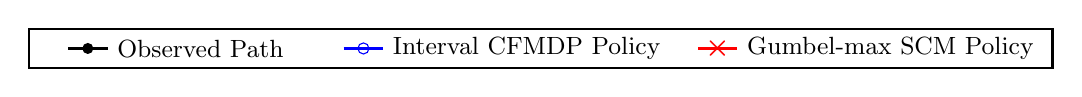
\begin{tikzpicture}[scale=1.0, every node/.style={scale=1.0}]
            \draw[thick, black] (-3, -0.25) rectangle (10, 0.25);
            %
            \draw[black, line width=1pt] (-2.5, 0.0) -- (-2,0.0);
            \fill[black] (-2.25,0.0) circle (2pt); %
            \node[right] at (-2,0.0) {\small Observed Path};
            
            %
            \draw[blue, line width=1pt] (1.0,0.0) -- (1.5,0.0);
            \node[draw=blue, circle, minimum size=4pt, inner sep=0pt] at (1.25,0.0) {}; %
            \node[right] at (1.5,0.0) {\small Interval CFMDP Policy};
            
            %
            \draw[red, line width=1pt] (5.5,0) -- (6,0);
            \node[red] at (5.75,0) {$\boldsymbol{\times}$}; %
            \node[right] at (6,0) {\small Gumbel-max SCM Policy};
        \end{tikzpicture}
    }\\
    %
    \subfigure[\footnotesize Lowest cumulative reward: Interval CFMDP ($312$), Gumbel-max SCM ($312$)]{%
        \resizebox{0.76\columnwidth}{!}{
             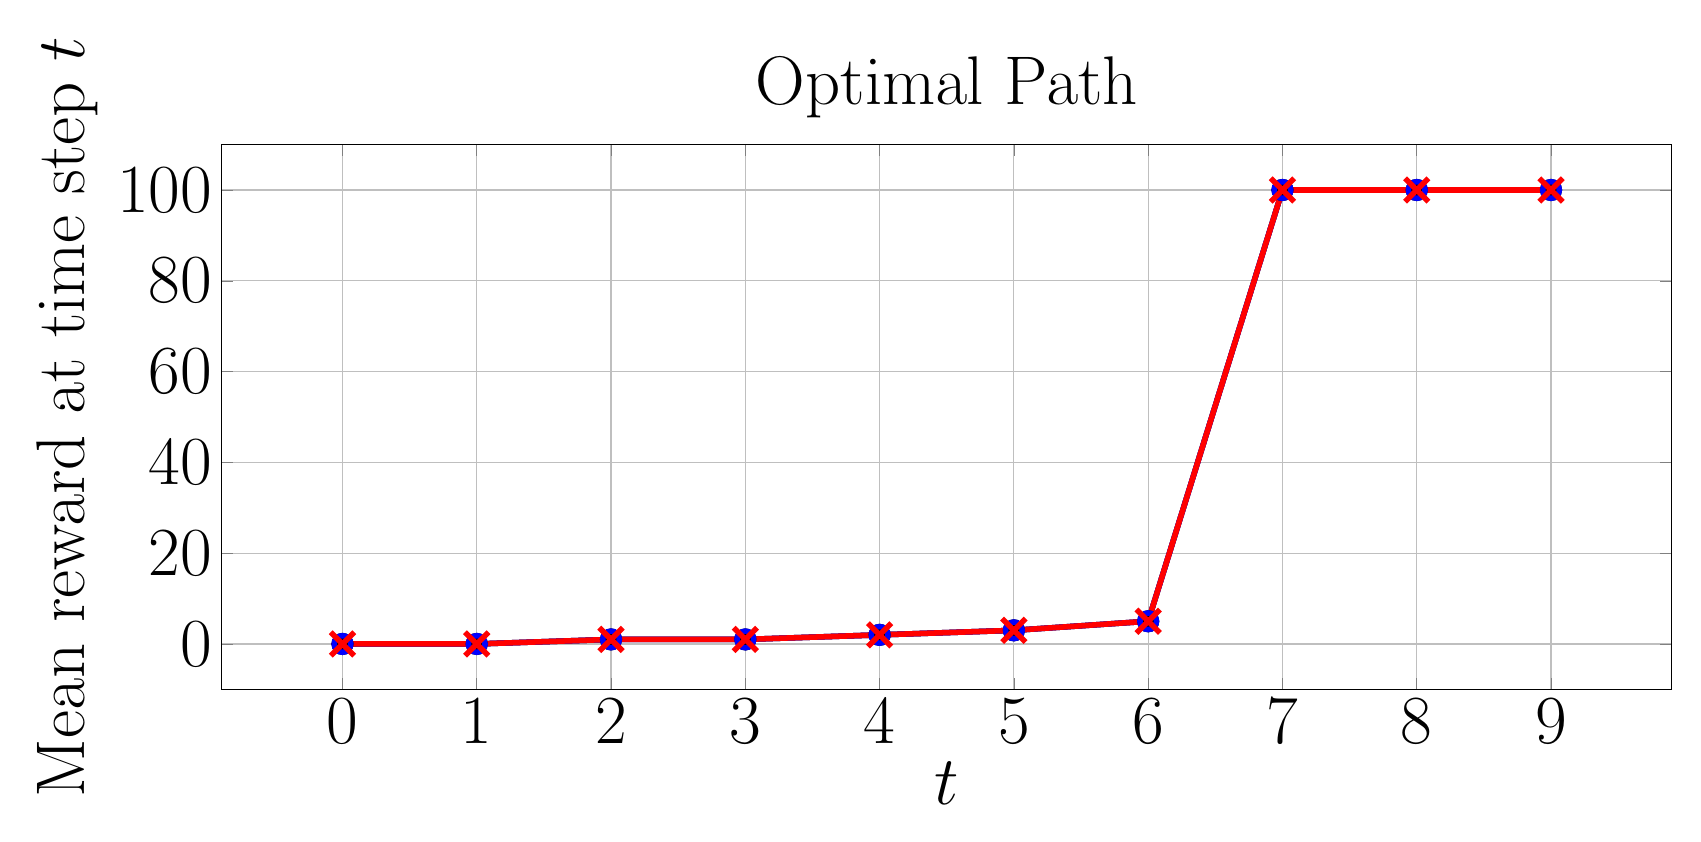
\begin{tikzpicture}
                \begin{axis}[
                    xlabel={$t$},
                    ylabel={Mean reward at time step $t$},
                    title={Optimal Path},
                    grid=both,
                    width=20cm, height=8.5cm,
                    every axis/.style={font=\Huge},
                    %
                ]
                \addplot[
                    color=black, %
                    mark=*, %
                    line width=2pt,
                    mark size=3pt,
                    error bars/.cd,
                    y dir=both, %
                    y explicit, %
                    error bar style={line width=1pt,solid},
                    error mark options={line width=1pt,mark size=4pt,rotate=90}
                ]
                coordinates {
                    (0, 0.0)  +- (0, 0.0)
                    (1, 0.0)  +- (0, 0.0) 
                    (2, 1.0)  +- (0, 0.0) 
                    (3, 1.0)  +- (0, 0.0)
                    (4, 2.0)  +- (0, 0.0)
                    (5, 3.0) +- (0, 0.0)
                    (6, 5.0) +- (0, 0.0)
                    (7, 100.0) +- (0, 0.0)
                    (8, 100.0) +- (0, 0.0)
                    (9, 100.0) +- (0, 0.0)
                };
                %
                \addplot[
                    color=blue, %
                    mark=o, %
                    line width=2pt,
                    mark size=3pt,
                    error bars/.cd,
                    y dir=both, %
                    y explicit, %
                    error bar style={line width=1pt,solid},
                    error mark options={line width=1pt,mark size=4pt,rotate=90}
                ]
                 coordinates {
                    (0, 0.0)  +- (0, 0.0)
                    (1, 0.0)  +- (0, 0.0) 
                    (2, 1.0)  +- (0, 0.0) 
                    (3, 1.0)  +- (0, 0.0)
                    (4, 2.0)  +- (0, 0.0)
                    (5, 3.0) +- (0, 0.0)
                    (6, 5.0) +- (0, 0.0)
                    (7, 100.0) +- (0, 0.0)
                    (8, 100.0) +- (0, 0.0)
                    (9, 100.0) +- (0, 0.0)
                };
                %
                \addplot[
                    color=red, %
                    mark=x, %
                    line width=2pt,
                    mark size=6pt,
                    error bars/.cd,
                    y dir=both, %
                    y explicit, %
                    error bar style={line width=1pt,solid},
                    error mark options={line width=1pt,mark size=4pt,rotate=90}
                ]
                coordinates {
                    (0, 0.0)  +- (0, 0.0)
                    (1, 0.0)  +- (0, 0.0) 
                    (2, 1.0)  +- (0, 0.0) 
                    (3, 1.0)  +- (0, 0.0)
                    (4, 2.0)  +- (0, 0.0)
                    (5, 3.0) +- (0, 0.0)
                    (6, 5.0) +- (0, 0.0)
                    (7, 100.0) +- (0, 0.0)
                    (8, 100.0) +- (0, 0.0)
                    (9, 100.0) +- (0, 0.0)
                };
                \end{axis}
            \end{tikzpicture}
         }
    }
    \hspace{1cm}
    \subfigure[\footnotesize Lowest cumulative reward: Interval CFMDP ($19$), Gumbel-max SCM ($-88$)]{%
         \resizebox{0.76\columnwidth}{!}{
            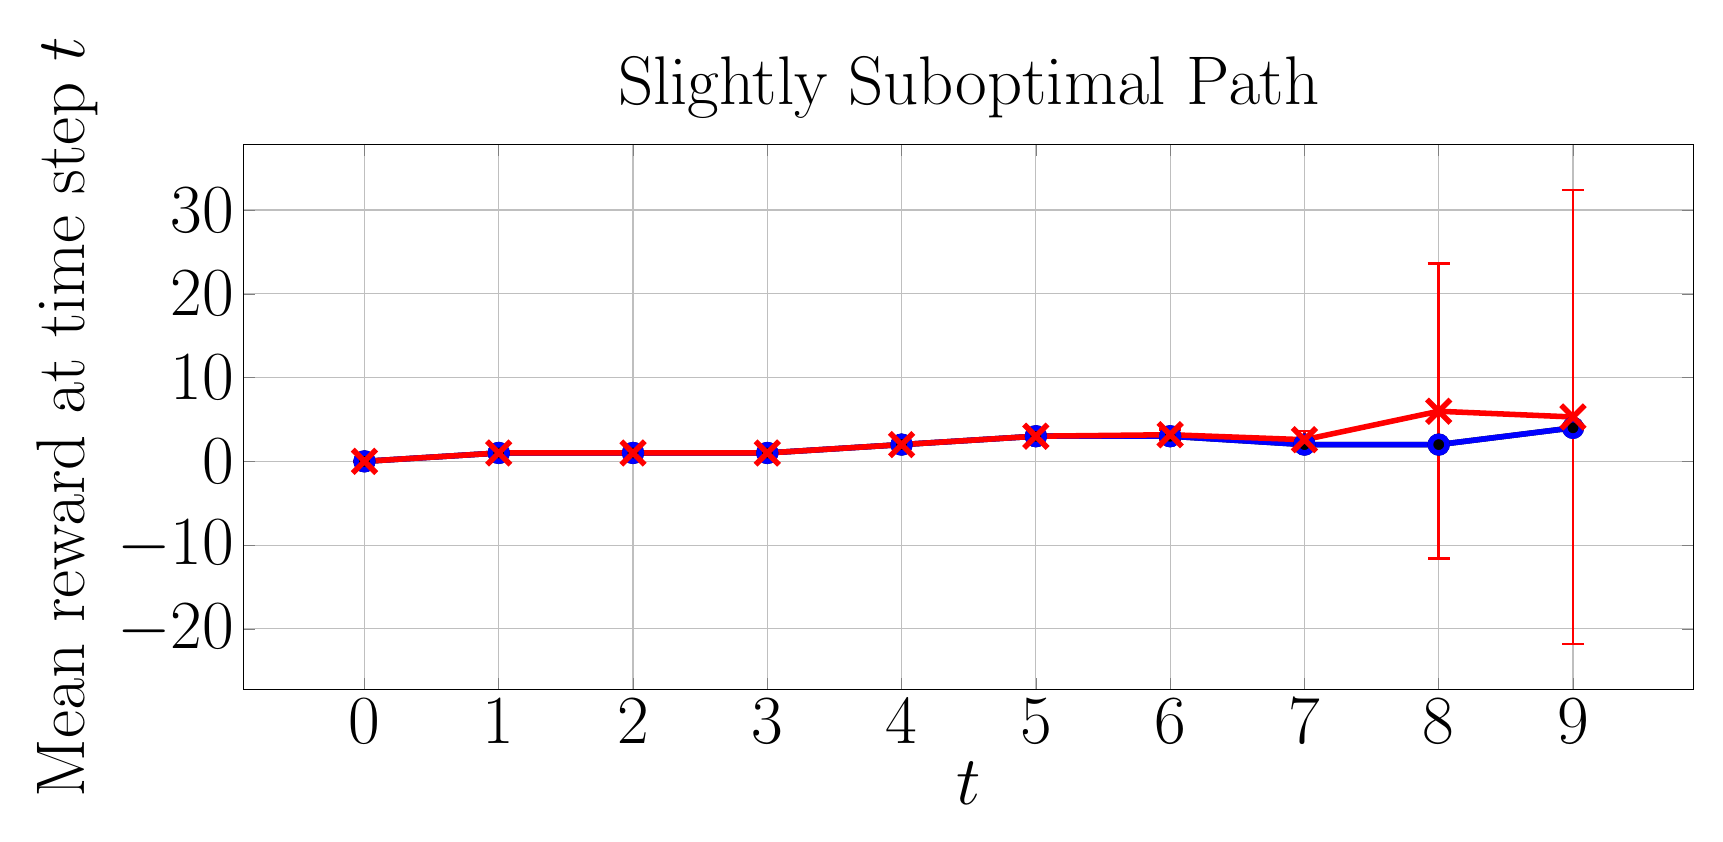
\begin{tikzpicture}
                \begin{axis}[
                    xlabel={$t$},
                    ylabel={Mean reward at time step $t$},
                    title={Slightly Suboptimal Path},
                    grid=both,
                    width=20cm, height=8.5cm,
                    every axis/.style={font=\Huge},
                    %
                ]
                \addplot[
                    color=black, %
                    mark=*, %
                    line width=2pt,
                    mark size=3pt,
                    error bars/.cd,
                    y dir=both, %
                    y explicit, %
                    error bar style={line width=1pt,solid},
                    error mark options={line width=1pt,mark size=4pt,rotate=90}
                ]
              coordinates {
                    (0, 0.0)  +- (0, 0.0)
                    (1, 1.0)  +- (0, 0.0) 
                    (2, 1.0)  +- (0, 0.0) 
                    (3, 1.0)  +- (0, 0.0)
                    (4, 2.0)  +- (0, 0.0)
                    (5, 3.0) +- (0, 0.0)
                    (6, 3.0) +- (0, 0.0)
                    (7, 2.0) +- (0, 0.0)
                    (8, 2.0) +- (0, 0.0)
                    (9, 4.0) +- (0, 0.0)
                };
                %
                \addplot[
                    color=blue, %
                    mark=o, %
                    line width=2pt,
                    mark size=3pt,
                    error bars/.cd,
                    y dir=both, %
                    y explicit, %
                    error bar style={line width=1pt,solid},
                    error mark options={line width=1pt,mark size=4pt,rotate=90}
                ]
              coordinates {
                    (0, 0.0)  +- (0, 0.0)
                    (1, 1.0)  +- (0, 0.0) 
                    (2, 1.0)  +- (0, 0.0) 
                    (3, 1.0)  +- (0, 0.0)
                    (4, 2.0)  +- (0, 0.0)
                    (5, 3.0) +- (0, 0.0)
                    (6, 3.0) +- (0, 0.0)
                    (7, 2.0) +- (0, 0.0)
                    (8, 2.0) +- (0, 0.0)
                    (9, 4.0) +- (0, 0.0)
                };
                %
                \addplot[
                    color=red, %
                    mark=x, %
                    line width=2pt,
                    mark size=6pt,
                    error bars/.cd,
                    y dir=both, %
                    y explicit, %
                    error bar style={line width=1pt,solid},
                    error mark options={line width=1pt,mark size=4pt,rotate=90}
                ]
                coordinates {
                    (0, 0.0)  +- (0, 0.0)
                    (1, 1.0)  +- (0, 0.0) 
                    (2, 1.0)  +- (0, 0.0) 
                    (3, 1.0)  +- (0, 0.0)
                    (4, 2.0)  += (0, 0.0)
                    (5, 3.0)  += (0, 0.0)
                    (6, 3.17847) += (0, 0.62606746) -= (0, 0.62606746)
                    (7, 2.5832885) += (0, 1.04598233) -= (0, 1.04598233)
                    (8, 5.978909) += (0, 17.60137623) -= (0, 17.60137623)
                    (9, 5.297059) += (0, 27.09227512) -= (0, 27.09227512)
                };
                \end{axis}
            \end{tikzpicture}
         }
    }\\[-1.5pt]
    \subfigure[\footnotesize Lowest cumulative reward: Interval CFMDP ($14$), Gumbel-max SCM ($-598$)]{%
         \resizebox{0.76\columnwidth}{!}{
             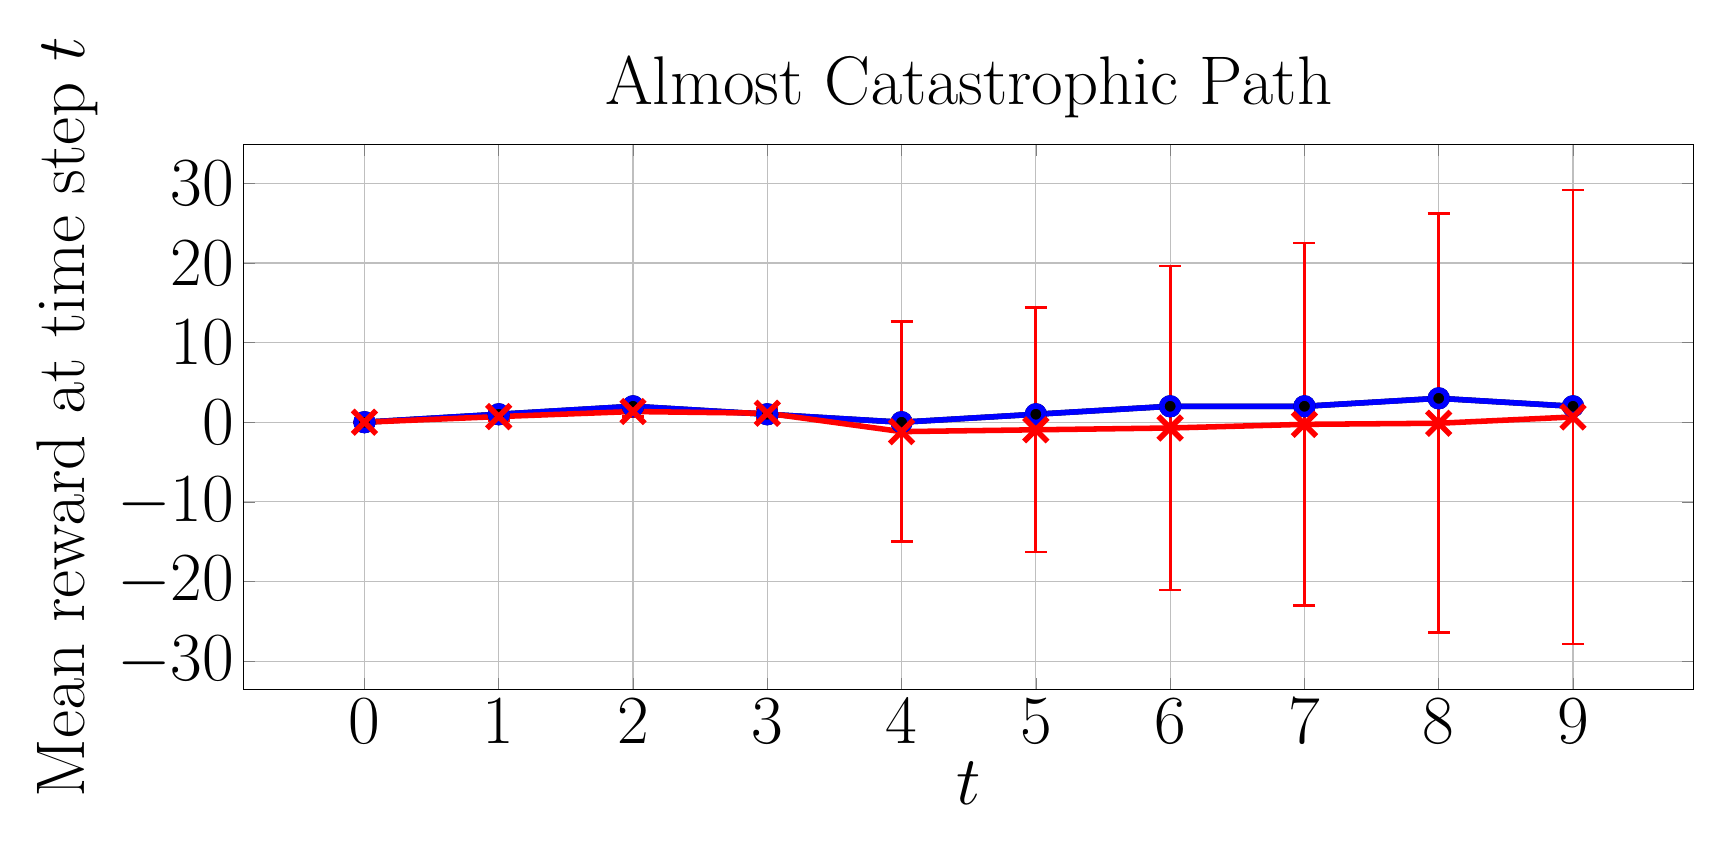
\begin{tikzpicture}
                \begin{axis}[
                    xlabel={$t$},
                    ylabel={Mean reward at time step $t$},
                    title={Almost Catastrophic Path},
                    grid=both,
                    width=20cm, height=8.5cm,
                    every axis/.style={font=\Huge},
                    %
                ]
                \addplot[
                    color=black, %
                    mark=*, %
                    line width=2pt,
                    mark size=3pt,
                    error bars/.cd,
                    y dir=both, %
                    y explicit, %
                    error bar style={line width=1pt,solid},
                    error mark options={line width=1pt,mark size=4pt,rotate=90}
                ]
                coordinates {
                    (0, 0.0)  +- (0, 0.0)
                    (1, 1.0)  +- (0, 0.0) 
                    (2, 2.0)  +- (0, 0.0) 
                    (3, 1.0)  +- (0, 0.0)
                    (4, 0.0)  +- (0, 0.0)
                    (5, 1.0) +- (0, 0.0)
                    (6, 2.0) +- (0, 0.0)
                    (7, 2.0) +- (0, 0.0)
                    (8, 3.0) +- (0, 0.0)
                    (9, 2.0) +- (0, 0.0)
                };
                %
                \addplot[
                    color=blue, %
                    mark=o, %
                    line width=2pt,
                    mark size=3pt,
                    error bars/.cd,
                    y dir=both, %
                    y explicit, %
                    error bar style={line width=1pt,solid},
                    error mark options={line width=1pt,mark size=4pt,rotate=90}
                ]
                coordinates {
                    (0, 0.0)  +- (0, 0.0)
                    (1, 1.0)  +- (0, 0.0) 
                    (2, 2.0)  +- (0, 0.0) 
                    (3, 1.0)  +- (0, 0.0)
                    (4, 0.0)  +- (0, 0.0)
                    (5, 1.0) +- (0, 0.0)
                    (6, 2.0) +- (0, 0.0)
                    (7, 2.0) +- (0, 0.0)
                    (8, 3.0) +- (0, 0.0)
                    (9, 2.0) +- (0, 0.0)
                };
                %
                \addplot[
                    color=red, %
                    mark=x, %
                    line width=2pt,
                    mark size=6pt,
                    error bars/.cd,
                    y dir=both, %
                    y explicit, %
                    error bar style={line width=1pt,solid},
                    error mark options={line width=1pt,mark size=4pt,rotate=90}
                ]
                coordinates {
                    (0, 0.0)  +- (0, 0.0)
                    (1, 0.7065655)  +- (0, 0.4553358) 
                    (2, 1.341673)  +- (0, 0.67091621) 
                    (3, 1.122926)  +- (0, 0.61281824)
                    (4, -1.1821935)  +- (0, 13.82444042)
                    (5, -0.952399)  +- (0, 15.35195457)
                    (6, -0.72672) +- (0, 20.33508414)
                    (7, -0.268983) +- (0, 22.77861454)
                    (8, -0.1310835) +- (0, 26.31013314)
                    (9, 0.65806) +- (0, 28.50670214)
                };
                %
            %
            %
            %
            %
            %
            %
            %
            %
            %
            %
            %
            %
            %
            %
            %
            %
            %
            %
                \end{axis}
            \end{tikzpicture}
         }
    }
    \hspace{1cm}
    \subfigure[\footnotesize Lowest cumulative reward: Interval CFMDP ($-698$), Gumbel-max SCM ($-698$)]{%
         \resizebox{0.76\columnwidth}{!}{
            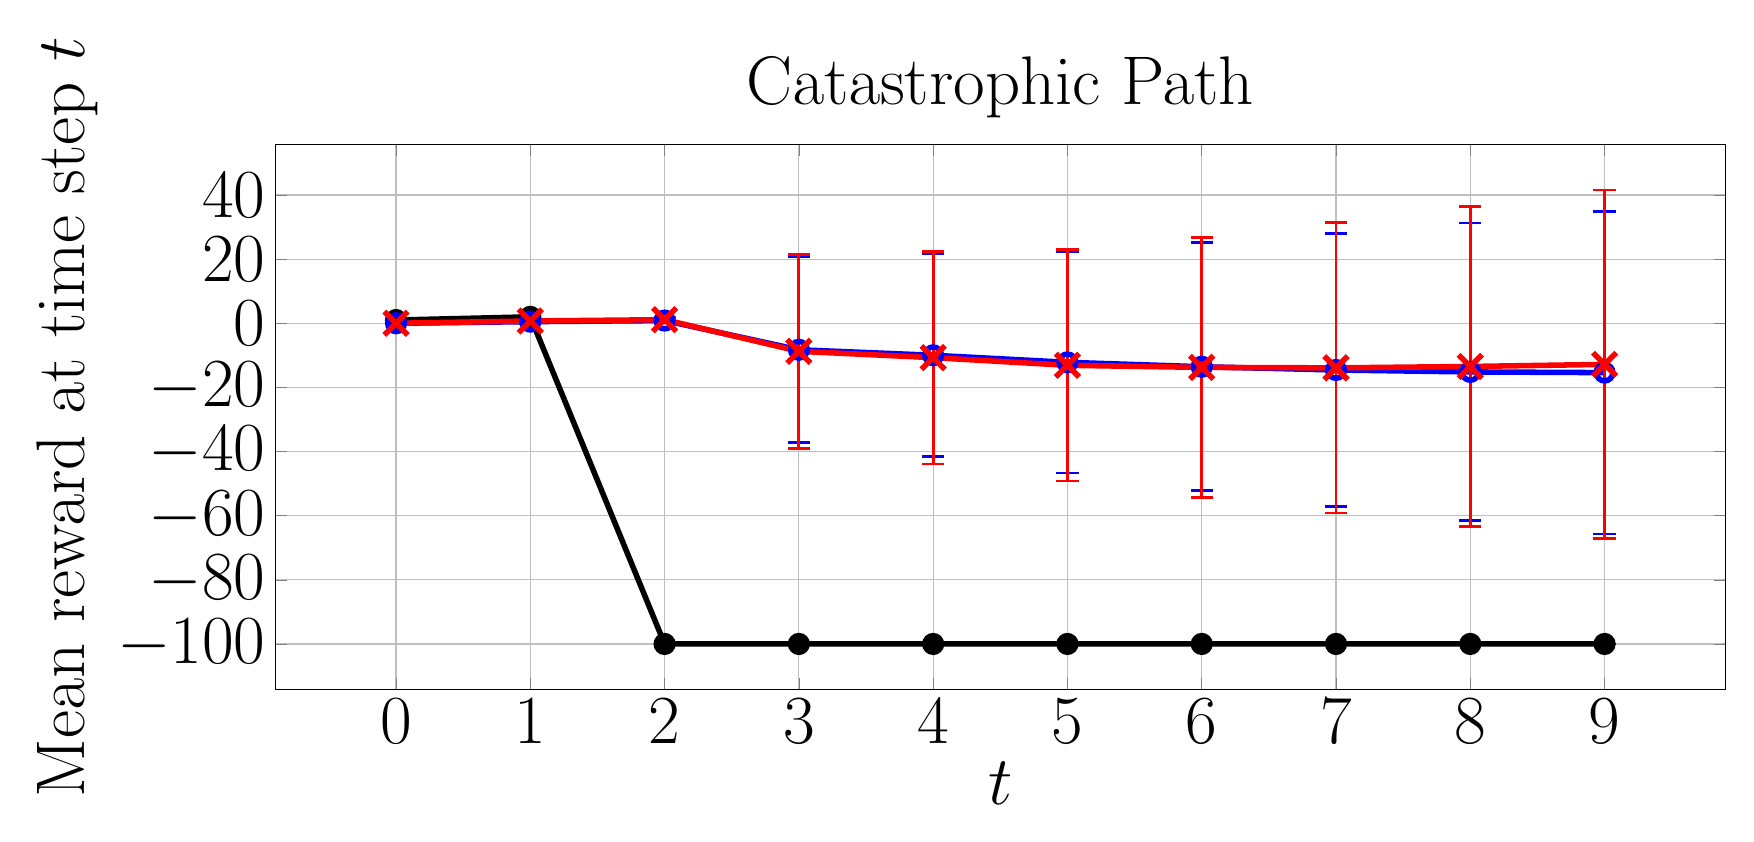
\begin{tikzpicture}
                \begin{axis}[
                    xlabel={$t$},
                    ylabel={Mean reward at time step $t$},
                    title={Catastrophic Path},
                    grid=both,
                    width=20cm, height=8.5cm,
                    every axis/.style={font=\Huge},
                    %
                ]
                \addplot[
                    color=black, %
                    mark=*, %
                    line width=2pt,
                    mark size=3pt,
                    error bars/.cd,
                    y dir=both, %
                    y explicit, %
                    error bar style={line width=1pt,solid},
                    error mark options={line width=1pt,mark size=4pt,rotate=90}
                ]
                coordinates {
                    (0, 1.0)  +- (0, 0.0)
                    (1, 2.0)  +- (0, 0.0) 
                    (2, -100.0)  +- (0, 0.0) 
                    (3, -100.0)  +- (0, 0.0)
                    (4, -100.0)  +- (0, 0.0)
                    (5, -100.0) +- (0, 0.0)
                    (6, -100.0) +- (0, 0.0)
                    (7, -100.0) +- (0, 0.0)
                    (8, -100.0) +- (0, 0.0)
                    (9, -100.0) +- (0, 0.0)
                };
                %
                \addplot[
                    color=blue, %
                    mark=o, %
                    line width=2pt,
                    mark size=3pt,
                    error bars/.cd,
                    y dir=both, %
                    y explicit, %
                    error bar style={line width=1pt,solid},
                    error mark options={line width=1pt,mark size=4pt,rotate=90}
                ]
                coordinates {
                    (0, 0.0)  +- (0, 0.0)
                    (1, 0.504814)  +- (0, 0.49997682) 
                    (2, 0.8439835)  +- (0, 0.76831917) 
                    (3, -8.2709165)  +- (0, 28.93656754)
                    (4, -9.981082)  +- (0, 31.66825363)
                    (5, -12.1776325) +- (0, 34.53463233)
                    (6, -13.556076) +- (0, 38.62845372)
                    (7, -14.574418) +- (0, 42.49603359)
                    (8, -15.1757075) +- (0, 46.41913968)
                    (9, -15.3900395) +- (0, 50.33563368)
                };
                %
                \addplot[
                    color=red, %
                    mark=x, %
                    line width=2pt,
                    mark size=6pt,
                    error bars/.cd,
                    y dir=both, %
                    y explicit, %
                    error bar style={line width=1pt,solid},
                    error mark options={line width=1pt,mark size=4pt,rotate=90}
                ]
                coordinates {
                    (0, 0.0)  +- (0, 0.0)
                    (1, 0.701873)  +- (0, 0.45743556) 
                    (2, 1.1227805)  +- (0, 0.73433129) 
                    (3, -8.7503255)  +- (0, 30.30257976)
                    (4, -10.722092)  +- (0, 33.17618589)
                    (5, -13.10721)  +- (0, 36.0648089)
                    (6, -13.7631645) +- (0, 40.56553451)
                    (7, -13.909043) +- (0, 45.23829402)
                    (8, -13.472517) +- (0, 49.96270296)
                    (9, -12.8278835) +- (0, 54.38618735)
                };
                %
            %
            %
            %
            %
            %
            %
            %
            %
            %
            %
            %
            %
            %
            %
            %
            %
            %
            %
                \end{axis}
            \end{tikzpicture}
         }
    }
    \caption{Average instant reward of CF paths induced by policies on GridWorld $p=0.4$.}
    \label{fig: reward p=0.4}
\end{figure*}

\subsection{Experimental Setup}
To compare policy performance, we measure the average rewards of counterfactual paths induced by our policy and the Gumbel-max policy by uniformly sampling $200$ counterfactual MDPs from the ICFMDP and generating $10,000$ counterfactual paths over each sampled CFMDP. \jl{Since the interval CFMDP depends on the observed path, we select $4$  paths of varying optimality to evaluate how the observed path impacts the performance of both policies: an optimal path, a slightly suboptimal path that could reach the optimal reward with a few changes, a catastrophic path that enters a catastrophic, terminal state with low reward, and an almost catastrophic path that was close to entering a catastrophic state.} When measuring the average probability bound widths and execution time needed to generate the ICFMDPs, we averaged over $20$ randomly generated observed paths
\footnote{Further training details are provided in Appendix \ref{app: training details}, and the code is provided at \href{https://github.com/ddv-lab/robust-cf-inference-in-MDPs}{https://github.com/ddv-lab/robust-cf-inference-in-MDPs}
%
%
.}.

\subsection{GridWorld}
\jl{The GridWorld MDP is a $4 \times 4$ grid where an agent must navigate from the top-left corner to the goal state in the bottom-right corner, avoiding a dangerous terminal state in the centre. At each time step, the agent can move up, down, left, or right, but there is a small probability (controlled by hyper-parameter $p$) of moving in an unintended direction. As the agent nears the goal, the reward for each state increases, culminating in a reward of $+100$ for reaching the goal. Entering the dangerous state results in a penalty of $-100$. We use two versions of GridWorld: a less stochastic version with $p=0.9$ (i.e., $90$\% chance of moving in the chosen direction) and a more stochastic version with $p=0.4$.}

\paragraph{GridWorld ($p=0.9$)}
When $p=0.9$, the counterfactual probability bounds are typically narrow (see Table \ref{tab:nonzero_probs} for average measurements). Consequently, as shown in Figure \ref{fig: reward p=0.9}, both policies are nearly identical and perform similarly well across the optimal, slightly suboptimal, and catastrophic paths.
%
However, for the almost catastrophic path, the interval CFMDP path is more conservative and follows the observed path more closely (as this is where the probability bounds are narrowest), which typically requires one additional step to reach the goal state than the Gumbel-max SCM policy.
%

\paragraph{GridWorld ($p=0.4$)}
\jl{When $p=0.4$, the GridWorld environment becomes more uncertain, increasing the risk of entering the dangerous state even if correct actions are chosen. Thus, as shown in Figure \ref{fig: reward p=0.4}, the interval CFMDP policy adopts a more conservative approach, avoiding deviation from the observed policy if it cannot guarantee higher counterfactual rewards (see the slightly suboptimal and almost catastrophic paths), whereas the Gumbel-max SCM is inconsistent: it can yield higher rewards, but also much lower rewards, reflected in the wide error bars.} For the catastrophic path, both policies must deviate from the observed path to achieve a higher reward and, in this case, perform similarly.
%
%
%
%
\subsection{Sepsis}
The Sepsis MDP \citep{oberst2019counterfactual} simulates trajectories of Sepsis patients. Each state consists of four vital signs (heart rate, blood pressure, oxygen concentration, and glucose levels), categorised as low, normal, or high.
and three treatments that can be toggled on/off at each time step (8 actions in total). Unlike \citet{oberst2019counterfactual}, we scale rewards based on the number of out-of-range vital signs, between $-1000$ (patient dies) and $1000$ (patient discharged). \jl{Like the GridWorld $p=0.4$ experiment, the Sepsis MDP is highly uncertain, as many states are equally likely to lead to optimal and poor outcomes. Thus, as shown in Figure \ref{fig: reward sepsis}, both policies follow the observed optimal and almost catastrophic paths to guarantee rewards are no worse than the observation.} However, improving the catastrophic path requires deviating from the observation. Here, the Gumbel-max SCM policy, on average, performs better than the interval CFMDP policy. But, since both policies have lower bounds clipped at $-1000$, neither policy reliably improves over the observation. In contrast, for the slightly suboptimal path, the interval CFMDP policy performs significantly better, shown by its higher lower bounds. 
Moreover, in these two cases, the worst-case counterfactual path generated by the interval CFMDP policy is better than that of the Gumbel-max SCM policy,
indicating its greater robustness.
%
\begin{figure*}
    \centering
     \resizebox{0.6\textwidth}{!}{
        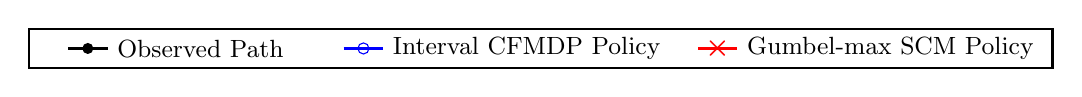
\begin{tikzpicture}[scale=1.0, every node/.style={scale=1.0}]
            \draw[thick, black] (-3, -0.25) rectangle (10, 0.25);
            %
            \draw[black, line width=1pt] (-2.5, 0.0) -- (-2,0.0);
            \fill[black] (-2.25,0.0) circle (2pt); %
            \node[right] at (-2,0.0) {\small Observed Path};
            
            %
            \draw[blue, line width=1pt] (1.0,0.0) -- (1.5,0.0);
            \node[draw=blue, circle, minimum size=4pt, inner sep=0pt] at (1.25,0.0) {}; %
            \node[right] at (1.5,0.0) {\small Interval CFMDP Policy};
            
            %
            \draw[red, line width=1pt] (5.5,0) -- (6,0);
            \node[red] at (5.75,0) {$\boldsymbol{\times}$}; %
            \node[right] at (6,0) {\small Gumbel-max SCM Policy};
        \end{tikzpicture}
    }\\
    \subfigure[\footnotesize Lowest cumulative reward: Interval CFMDP ($8000$), Gumbel-max SCM ($8000$)]{%
         \resizebox{0.76\columnwidth}{!}{
             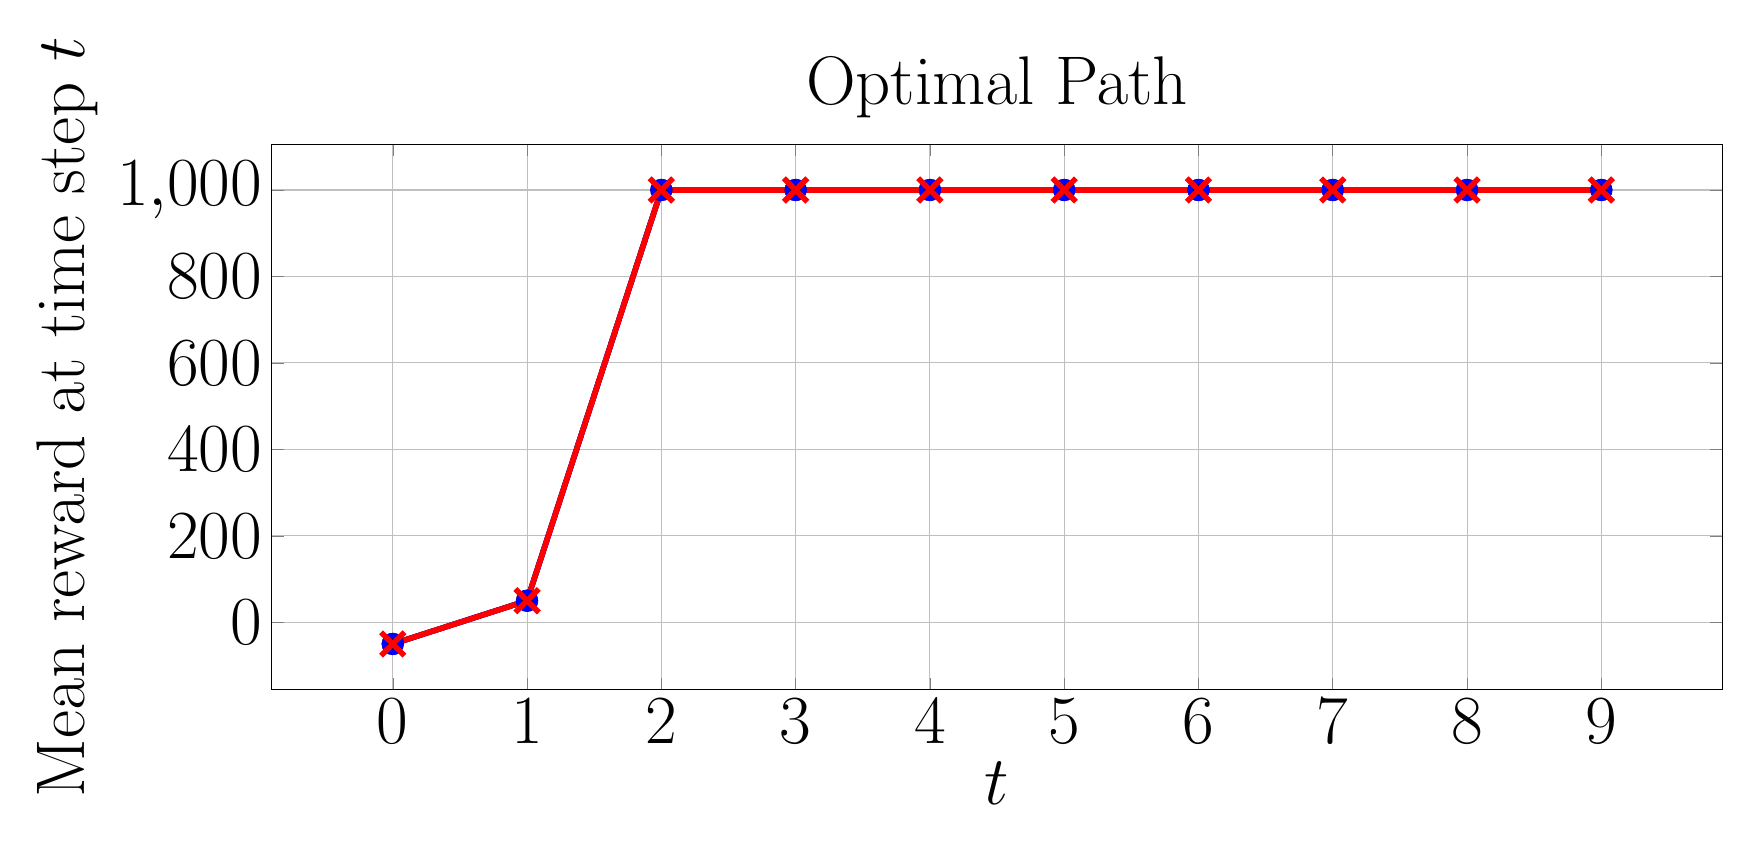
\begin{tikzpicture}
                \begin{axis}[
                    xlabel={$t$},
                    ylabel={Mean reward at time step $t$},
                    title={Optimal Path},
                    grid=both,
                    width=20cm, height=8.5cm,
                    every axis/.style={font=\Huge},
                    %
                ]
                \addplot[
                    color=black, %
                    mark=*, %
                    line width=2pt,
                    mark size=3pt,
                ]
                coordinates {
                    (0, -50.0)
                    (1, 50.0)
                    (2, 1000.0)
                    (3, 1000.0)
                    (4, 1000.0)
                    (5, 1000.0)
                    (6, 1000.0)
                    (7, 1000.0)
                    (8, 1000.0)
                    (9, 1000.0)
                };
                %
                \addplot[
                    color=blue, %
                    mark=o, %
                    line width=2pt,
                    mark size=3pt,
                    error bars/.cd,
                    y dir=both, %
                    y explicit, %
                    error bar style={line width=1pt,solid},
                    error mark options={line width=1pt,mark size=4pt,rotate=90}
                ]
                coordinates {
                    (0, -50.0)  +- (0, 0.0)
                    (1, 50.0)  +- (0, 0.0) 
                    (2, 1000.0)  +- (0, 0.0) 
                    (3, 1000.0)  +- (0, 0.0)
                    (4, 1000.0)  +- (0, 0.0)
                    (5, 1000.0) +- (0, 0.0)
                    (6, 1000.0) +- (0, 0.0)
                    (7, 1000.0) +- (0, 0.0)
                    (8, 1000.0) +- (0, 0.0)
                    (9, 1000.0) +- (0, 0.0)
                };
                %
                \addplot[
                    color=red, %
                    mark=x, %
                    line width=2pt,
                    mark size=6pt,
                    error bars/.cd,
                    y dir=both, %
                    y explicit, %
                    error bar style={line width=1pt,solid},
                    error mark options={line width=1pt,mark size=4pt,rotate=90}
                ]
                coordinates {
                    (0, -50.0)  +- (0, 0.0)
                    (1, 50.0)  +- (0, 0.0) 
                    (2, 1000.0)  +- (0, 0.0) 
                    (3, 1000.0)  +- (0, 0.0)
                    (4, 1000.0)  +- (0, 0.0)
                    (5, 1000.0) +- (0, 0.0)
                    (6, 1000.0) +- (0, 0.0)
                    (7, 1000.0) +- (0, 0.0)
                    (8, 1000.0) +- (0, 0.0)
                    (9, 1000.0) +- (0, 0.0)
                };
                %
                \end{axis}
            \end{tikzpicture}
         }
    }
    \hspace{1cm}
    \subfigure[\footnotesize Lowest cumulative reward: Interval CFMDP ($-5980$), Gumbel-max SCM ($-8000$)]{%
         \resizebox{0.76\columnwidth}{!}{
            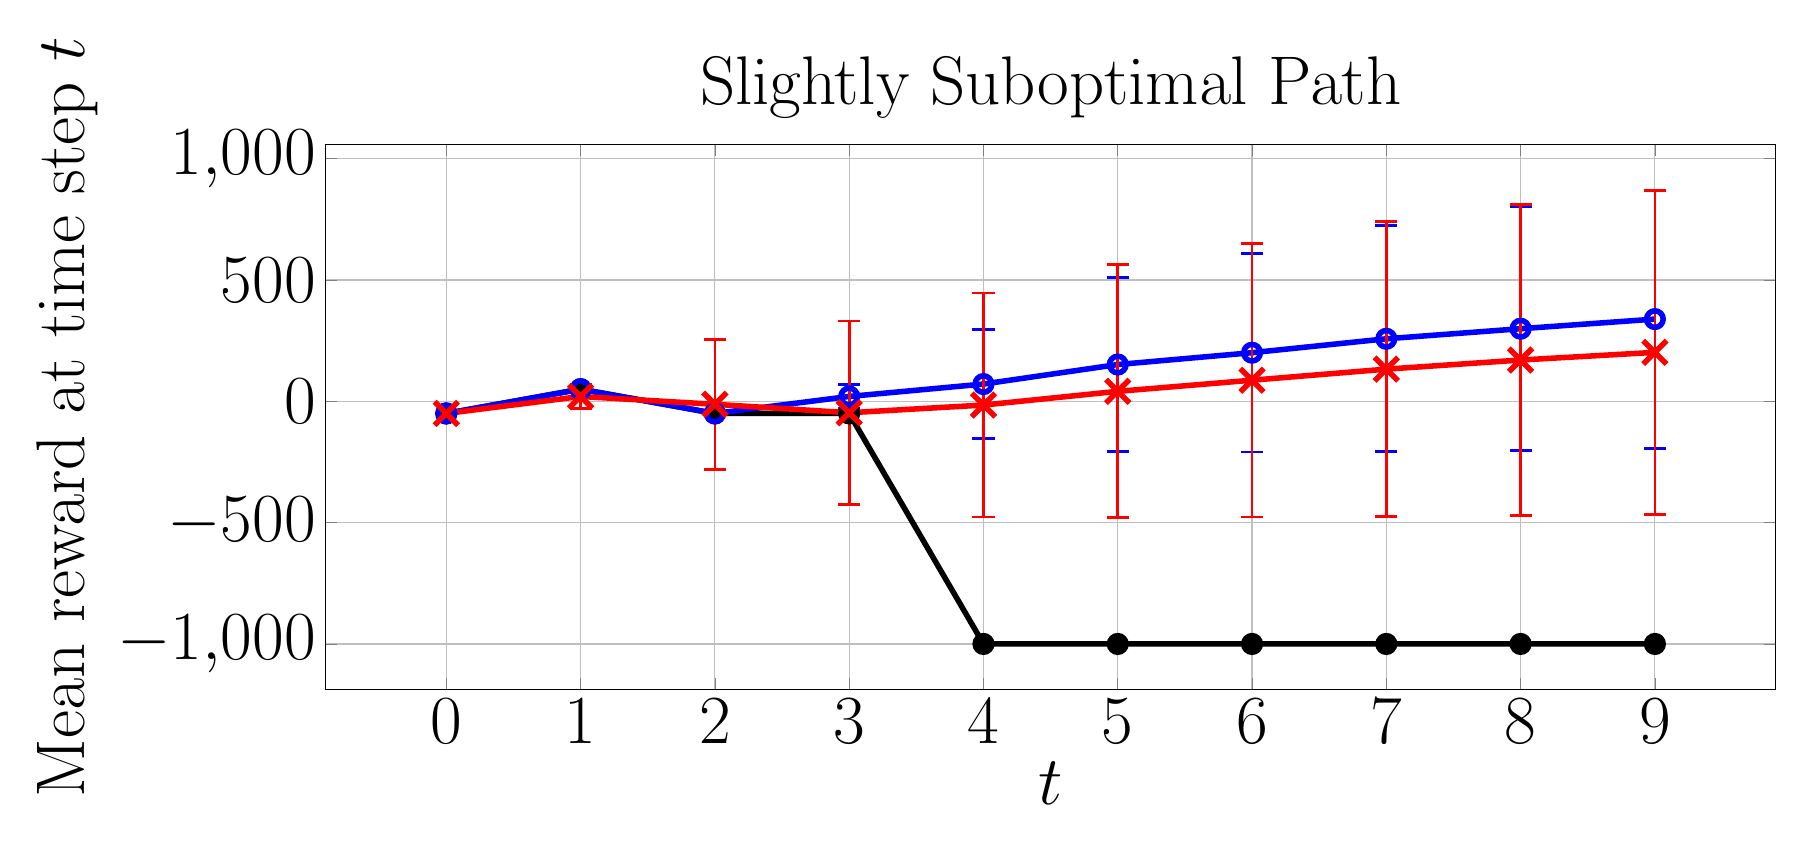
\begin{tikzpicture}
                \begin{axis}[
                    xlabel={$t$},
                    ylabel={Mean reward at time step $t$},
                    title={Slightly Suboptimal Path},
                    grid=both,
                    width=20cm, height=8.5cm,
                    every axis/.style={font=\Huge},
                    %
                ]
               \addplot[
                    color=black, %
                    mark=*, %
                    line width=2pt,
                    mark size=3pt,
                ]
                coordinates {
                    (0, -50.0)
                    (1, 50.0)
                    (2, -50.0)
                    (3, -50.0)
                    (4, -1000.0)
                    (5, -1000.0)
                    (6, -1000.0)
                    (7, -1000.0)
                    (8, -1000.0)
                    (9, -1000.0)
                };
                %
                \addplot[
                    color=blue, %
                    mark=o, %
                    line width=2pt,
                    mark size=3pt,
                    error bars/.cd,
                    y dir=both, %
                    y explicit, %
                    error bar style={line width=1pt,solid},
                    error mark options={line width=1pt,mark size=4pt,rotate=90}
                ]
                coordinates {
                    (0, -50.0)  +- (0, 0.0)
                    (1, 50.0)  +- (0, 0.0) 
                    (2, -50.0)  +- (0, 0.0) 
                    (3, 20.0631)  +- (0, 49.97539413)
                    (4, 71.206585)  +- (0, 226.02033693)
                    (5, 151.60797) +- (0, 359.23292559)
                    (6, 200.40593) +- (0, 408.86185176)
                    (7, 257.77948) +- (0, 466.10372804)
                    (8, 299.237465) +- (0, 501.82579506)
                    (9, 338.9129) +- (0, 532.06124996)
                };
                %
                \addplot[
                    color=red, %
                    mark=x, %
                    line width=2pt,
                    mark size=6pt,
                    error bars/.cd,
                    y dir=both, %
                    y explicit, %
                    error bar style={line width=1pt,solid},
                    error mark options={line width=1pt,mark size=4pt,rotate=90}
                ]
                coordinates {
                    (0, -50.0)  +- (0, 0.0)
                    (1, 20.00736)  +- (0, 49.99786741) 
                    (2, -12.282865)  +- (0, 267.598755) 
                    (3, -47.125995)  +- (0, 378.41755832)
                    (4, -15.381965)  +- (0, 461.77616558)
                    (5, 41.15459) +- (0, 521.53189262)
                    (6, 87.01595) +- (0, 564.22243126 )
                    (7, 132.62376) +- (0, 607.31338037)
                    (8, 170.168145) +- (0, 641.48013693)
                    (9, 201.813135) +- (0, 667.29441777)
                };
                %
                %
                %
                %
                %
                %
                %
                %
                %
                %
                %
                %
                %
                %
                %
                %
                %
                %
                %
                \end{axis}
            \end{tikzpicture}
         }
    }\\[-1.5pt]
    \subfigure[\footnotesize Lowest cumulative reward: Interval CFMDP ($100$), Gumbel-max SCM ($100$)]{%
         \resizebox{0.76\columnwidth}{!}{
             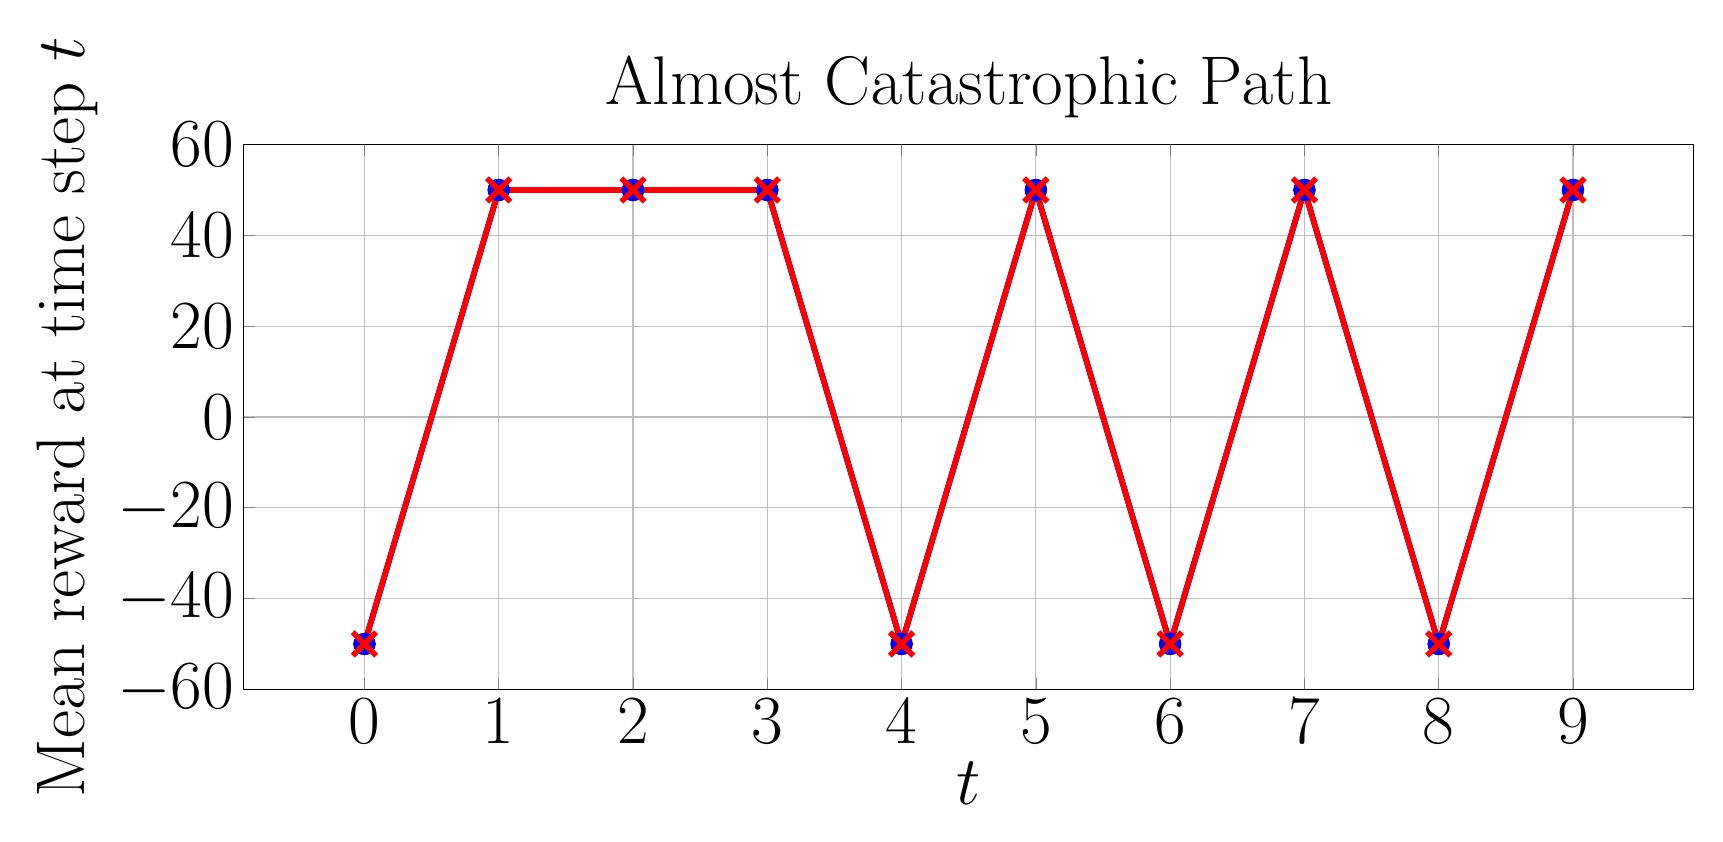
\begin{tikzpicture}
                \begin{axis}[
                    xlabel={$t$},
                    ylabel={Mean reward at time step $t$},
                    title={Almost Catastrophic Path},
                    grid=both,
                    every axis/.style={font=\Huge},
                    width=20cm, height=8.5cm,
                    %
                ]
               \addplot[
                    color=black, %
                    mark=*, %
                    line width=2pt,
                    mark size=3pt,
                ]
                coordinates {
                    (0, -50.0)
                    (1, 50.0)
                    (2, 50.0)
                    (3, 50.0)
                    (4, -50.0)
                    (5, 50.0)
                    (6, -50.0)
                    (7, 50.0)
                    (8, -50.0)
                    (9, 50.0)
                };
                %
                %
                \addplot[
                    color=blue, %
                    mark=o, %
                    line width=2pt,
                    mark size=3pt,
                    error bars/.cd,
                    y dir=both, %
                    y explicit, %
                    error bar style={line width=1pt,solid},
                    error mark options={line width=1pt,mark size=4pt,rotate=90}
                ]
                coordinates {
                    (0, -50.0)  +- (0, 0.0)
                    (1, 50.0)  +- (0, 0.0) 
                    (2, 50.0)  +- (0, 0.0) 
                    (3, 50.0)  +- (0, 0.0)
                    (4, -50.0)  +- (0, 0.0)
                    (5, 50.0) +- (0, 0.0)
                    (6, -50.0) +- (0, 0.0)
                    (7, 50.0) +- (0, 0.0)
                    (8, -50.0) +- (0, 0.0)
                    (9, 50.0) +- (0, 0.0)
                };
                %
                \addplot[
                    color=red, %
                    mark=x, %
                    line width=2pt,
                    mark size=6pt,
                    error bars/.cd,
                    y dir=both, %
                    y explicit, %
                    error bar style={line width=1pt,solid},
                    error mark options={line width=1pt,mark size=4pt,rotate=90}
                ]
                coordinates {
                    (0, -50.0)  +- (0, 0.0)
                    (1, 50.0)  +- (0, 0.0) 
                    (2, 50.0)  +- (0, 0.0) 
                    (3, 50.0)  +- (0, 0.0)
                    (4, -50.0)  +- (0, 0.0)
                    (5, 50.0) +- (0, 0.0)
                    (6, -50.0) +- (0, 0.0)
                    (7, 50.0) +- (0, 0.0)
                    (8, -50.0) +- (0, 0.0)
                    (9, 50.0) +- (0, 0.0)
                };
                %
                %
                %
                %
                %
                %
                %
                %
                %
                %
                %
                %
                %
                %
                %
                %
                %
                %
                %
                \end{axis}
            \end{tikzpicture}
         }
    }
    \hspace{1cm}
    \subfigure[\footnotesize Lowest cumulative reward: Interval CFMDP ($-7150$), Gumbel-max SCM ($-9050$)]{%
         \resizebox{0.76\columnwidth}{!}{
            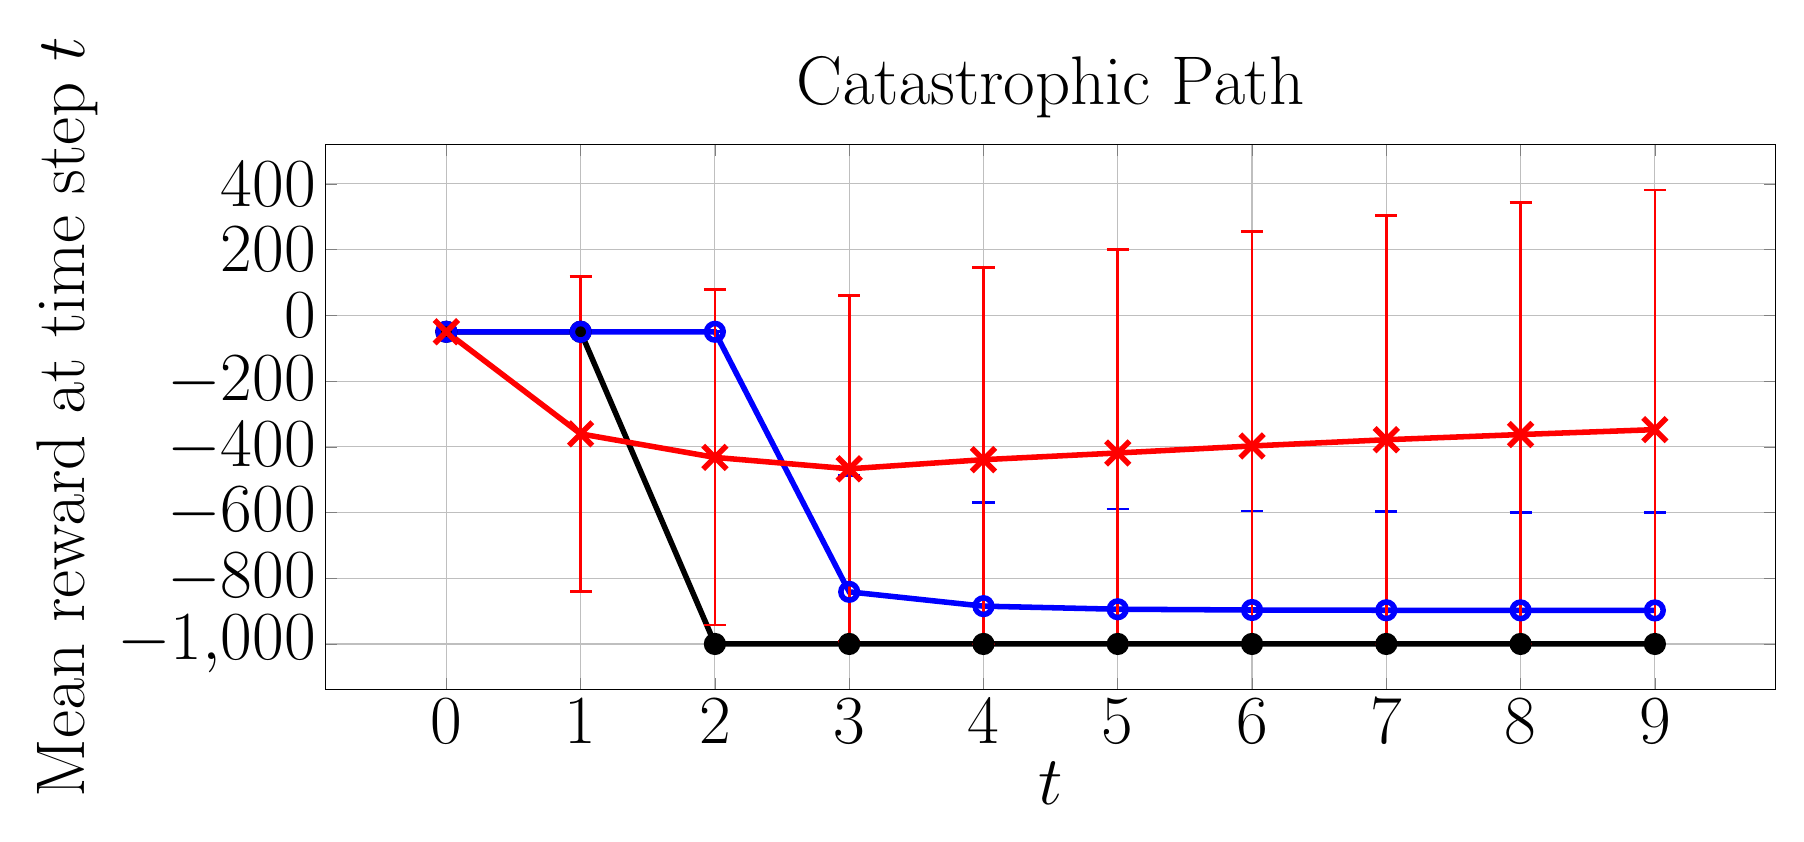
\begin{tikzpicture}
                \begin{axis}[
                    xlabel={$t$},
                    ylabel={Mean reward at time step $t$},
                    title={Catastrophic Path},
                    grid=both,
                    width=20cm, height=8.5cm,
                    every axis/.style={font=\Huge},
                    %
                ]
               \addplot[
                    color=black, %
                    mark=*, %
                    line width=2pt,
                    mark size=3pt,
                ]
                coordinates {
                    (0, -50.0)
                    (1, -50.0)
                    (2, -1000.0)
                    (3, -1000.0)
                    (4, -1000.0)
                    (5, -1000.0)
                    (6, -1000.0)
                    (7, -1000.0)
                    (8, -1000.0)
                    (9, -1000.0)
                };
                %
                %
                \addplot[
                    color=blue, %
                    mark=o, %
                    line width=2pt,
                    mark size=3pt,
                    error bars/.cd,
                    y dir=both, %
                    y explicit, %
                    error bar style={line width=1pt,solid},
                    error mark options={line width=1pt,mark size=4pt,rotate=90}
                ]
                coordinates {
                    (0, -50.0)  +- (0, 0.0)
                    (1, -50.0)  +- (0, 0.0) 
                    (2, -50.0)  +- (0, 0.0) 
                    (3, -841.440725)  += (0, 354.24605512) -= (0, 158.559275)
                    (4, -884.98225)  += (0, 315.37519669) -= (0, 115.01775)
                    (5, -894.330425) += (0, 304.88572805) -= (0, 105.669575)
                    (6, -896.696175) += (0, 301.19954514) -= (0, 103.303825)
                    (7, -897.4635) += (0, 299.61791279) -= (0, 102.5365)
                    (8, -897.77595) += (0, 298.80392585) -= (0, 102.22405)
                    (9, -897.942975) += (0, 298.32920557) -= (0, 102.057025)
                };
                %
                \addplot[
                    color=red, %
                    mark=x, %
                    line width=2pt,
                    mark size=6pt,
                    error bars/.cd,
                    y dir=both, %
                    y explicit, %
                    error bar style={line width=1pt,solid},
                    error mark options={line width=1pt,mark size=4pt,rotate=90}
                ]
            coordinates {
                    (0, -50.0)  +- (0, 0.0)
                    (1, -360.675265)  +- (0, 479.39812699) 
                    (2, -432.27629)  +- (0, 510.38620897) 
                    (3, -467.029545)  += (0, 526.36009628) -= (0, 526.36009628)
                    (4, -439.17429)  += (0, 583.96638919) -= (0, 560.82571)
                    (5, -418.82704) += (0, 618.43027478) -= (0, 581.17296)
                    (6, -397.464895) += (0, 652.67322574) -= (0, 602.535105)
                    (7, -378.49052) += (0, 682.85407033) -= (0, 621.50948)
                    (8, -362.654195) += (0, 707.01412023) -= (0, 637.345805)
                    (9, -347.737935) += (0, 729.29076479) -= (0, 652.262065)
                };
                %
                %
                %
                %
                %
                %
                %
                %
                %
                %
                %
                %
                %
                %
                %
                %
                %
                %
                %
                \end{axis}
            \end{tikzpicture}
         }
    }
    \caption{Average instant reward of CF paths induced by policies on Sepsis.}
    \label{fig: reward sepsis}
\end{figure*}

%
%
%
\subsection{Interval CFMDP Bounds}
%
%
Table \ref{tab:nonzero_probs} presents the mean counterfactual probability bound widths (excluding transitions where the upper bound is $0$) for each MDP, averaged over 20 observed paths. We compare the bounds under counterfactual stability (CS) and monotonicity (M) assumptions, CS alone, and no assumptions. This shows that the assumptions marginally reduce the bound widths, indicating the assumptions tighten the bounds without excluding too many causal models, as intended.
\renewcommand{\arraystretch}{1}

\begin{table}
\centering
\caption{Mean width of counterfactual probability bounds}
\resizebox{0.8\columnwidth}{!}{%
\begin{tabular}{|c|c|c|c|}
\hline
\multirow{2}{*}{\textbf{Environment}} & \multicolumn{3}{c|}{\textbf{Assumptions}} \\ \cline{2-4}
 & \textbf{CS + M} & \textbf{CS} & \textbf{None\tablefootnote{\jl{Equivalent to \citet{li2024probabilities}'s bounds (see Section \ref{sec: equivalence with Li}).}}} \\ \hline
\textbf{GridWorld} ($p=0.9$) & 0.0817 & 0.0977 & 0.100 \\ \hline
\textbf{GridWorld} ($p=0.4$) & 0.552  & 0.638  & 0.646 \\ \hline
\textbf{Sepsis} & 0.138 & 0.140 & 0.140 \\ \hline
\end{tabular}
}
\label{tab:nonzero_probs}
\end{table}


\subsection{Execution Times}
Table \ref{tab: times} compares the average time needed to generate the interval CFMDP vs.\ the Gumbel-max SCM CFMDP for 20 observations.
The GridWorld algorithms were run single-threaded, while the Sepsis experiments were run in parallel.
Generating the interval CFMDP is significantly faster as it uses exact analytical bounds, whereas the Gumbel-max CFMDP requires sampling from the Gumbel distribution to estimate counterfactual transition probabilities. \jl{Since constructing the counterfactual MDP models is the main bottleneck in both approaches, ours is more efficient overall and suitable for larger MDPs.}
\begin{table}
\centering
\caption{Mean execution time to generate CFMDPs}
\resizebox{0.99\columnwidth}{!}{%
\begin{tabular}{|c|c|c|}
\hline
\multirow{2}{*}{\textbf{Environment}} & \multicolumn{2}{c|}{\textbf{Mean Execution Time (s)}} \\ \cline{2-3} 
                                      & \textbf{Interval CFMDP} & \textbf{Gumbel-max CFMDP} \\ \hline
\textbf{GridWorld ($p=0.9$) }                  & 0.261                   & 56.1                      \\ \hline
\textbf{GridWorld ($p=0.4$)  }                 & 0.336                   & 54.5                      \\ \hline
\textbf{Sepsis}                                 & 688                     & 2940                      \\ \hline
\end{tabular}%
}
\label{tab: times}
\end{table}


%\section{Related Work}
%\label{sec:related-work}

%\subsection{Background}

%Defect detection is critical to ensure the yield of integrated circuit manufacturing lines and reduce faults. Previous research has primarily focused on wafer map data, which engineers produce by marking faulty chips with different colors based on test results. The specific spatial distribution of defects on a wafer can provide insights into the causes, thereby helping to determine which stage of the manufacturing process is responsible for the issues. Although such research is relatively mature, the continual miniaturization of integrated circuits and the increasing complexity and density of chip components have made chip-level detection more challenging, leading to potential risks\cite{ma2023review}. Consequently, there is a need to combine this approach with magnified imaging of the wafer surface using scanning electron microscopes (SEMs) to detect, classify, and analyze specific microscopic defects, thus helping to identify the particular process steps where defects originate.

%Previously, wafer surface defect classification and detection were primarily conducted by experienced engineers. However, this method relies heavily on the engineers' expertise and involves significant time expenditure and subjectivity, lacking uniform standards. With the ongoing development of artificial intelligence, deep learning methods using multi-layer neural networks to extract and learn target features have proven highly effective for this task\cite{gao2022review}.

%In the task of defect classification, it is typical to use a model structure that initially extracts features through convolutional and pooling layers, followed by classification via fully connected layers. Researchers have recently developed numerous classification model structures tailored to specific problems. These models primarily focus on how to extract defect features effectively. For instance, Chen et al. presented a defect recognition and classification algorithm rooted in PCA and classification SVM\cite{chen2008defect}. Chang et al. utilized SVM, drawing on features like smoothness and texture intricacy, for classifying high-intensity defect images\cite{chang2013hybrid}. The classification of defect images requires the formulation of numerous classifiers tailored for myriad inspection steps and an Abundance of accurately labeled data, making data acquisition challenging. Cheon et al. proposed a single CNN model adept at feature extraction\cite{cheon2019convolutional}. They achieved a granular classification of wafer surface defects by recognizing misclassified images and employing a k-nearest neighbors (k-NN) classifier algorithm to gauge the aggregate squared distance between each image feature vector and its k-neighbors within the same category. However, when applied to new or unseen defects, such models necessitate retraining, incurring computational overheads. Moreover, with escalating CNN complexity, the computational demands surge.

%Segmentation of defects is necessary to locate defect positions and gather information such as the size of defects. Unlike classification networks, segmentation networks often use classic encoder-decoder structures such as UNet\cite{ronneberger2015u} and SegNet\cite{badrinarayanan2017segnet}, which focus on effectively leveraging both local and global feature information. Han Hui et al. proposed integrating a Region Proposal Network (RPN) with a UNet architecture to suggest defect areas before conducting defect segmentation \cite{han2020polycrystalline}. This approach enables the segmentation of various defects in wafers with only a limited set of roughly labeled images, enhancing the efficiency of training and application in environments where detailed annotations are scarce. Subhrajit Nag et al. introduced a new network structure, WaferSegClassNet, which extracts multi-scale local features in the encoder and performs classification and segmentation tasks in the decoder \cite{nag2022wafersegclassnet}. This model represents the first detection system capable of simultaneously classifying and segmenting surface defects on wafers. However, it relies on extensive data training and annotation for high accuracy and reliability. 

%Recently, Vic De Ridder et al. introduced a novel approach for defect segmentation using diffusion models\cite{de2023semi}. This approach treats the instance segmentation task as a denoising process from noise to a filter, utilizing diffusion models to predict and reconstruct instance masks for semiconductor defects. This method achieves high precision and improved defect classification and segmentation detection performance. However, the complex network structure and the computational process of the diffusion model require substantial computational resources. Moreover, the performance of this model heavily relies on high-quality and large amounts of training data. These issues make it less suitable for industrial applications. Additionally, the model has only been applied to detecting and segmenting a single type of defect(bridges) following a specific manufacturing process step, limiting its practical utility in diverse industrial scenarios.

%\subsection{Few-shot Anomaly Detection}
%Traditional anomaly detection techniques typically rely on extensive training data to train models for identifying and locating anomalies. However, these methods often face limitations in rapidly changing production environments and diverse anomaly types. Recent research has started exploring effective anomaly detection using few or zero samples to address these challenges.

%Huang et al. developed the anomaly detection method RegAD, based on image registration technology. This method pre-trains an object-agnostic registration network with various images to establish the normality of unseen objects. It identifies anomalies by aligning image features and has achieved promising results. Despite these advancements, implementing few-shot settings in anomaly detection remains an area ripe for further exploration. Recent studies show that pre-trained vision-language models such as CLIP and MiniGPT can significantly enhance performance in anomaly detection tasks.

%Dong et al. introduced the MaskCLIP framework, which employs masked self-distillation to enhance contrastive language-image pretraining\cite{zhou2022maskclip}. This approach strengthens the visual encoder's learning of local image patches and uses indirect language supervision to enhance semantic understanding. It significantly improves transferability and pretraining outcomes across various visual tasks, although it requires substantial computational resources.
%Jeong et al. crafted the WinCLIP framework by integrating state words and prompt templates to characterize normal and anomalous states more accurately\cite{Jeong_2023_CVPR}. This framework introduces a novel window-based technique for extracting and aggregating multi-scale spatial features, significantly boosting the anomaly detection performance of the pre-trained CLIP model.
%Subsequently, Li et al. have further contributed to the field by creating a new expansive multimodal model named Myriad\cite{li2023myriad}. This model, which incorporates a pre-trained Industrial Anomaly Detection (IAD) model to act as a vision expert, embeds anomaly images as tokens interpretable by the language model, thus providing both detailed descriptions and accurate anomaly detection capabilities.
%Recently, Chen et al. introduced CLIP-AD\cite{chen2023clip}, and Li et al. proposed PromptAD\cite{li2024promptad}, both employing language-guided, tiered dual-path model structures and feature manipulation strategies. These approaches effectively address issues encountered when directly calculating anomaly maps using the CLIP model, such as reversed predictions and highlighting irrelevant areas. Specifically, CLIP-AD optimizes the utilization of multi-layer features, corrects feature misalignment, and enhances model performance through additional linear layer fine-tuning. PromptAD connects normal prompts with anomaly suffixes to form anomaly prompts, enabling contrastive learning in a single-class setting.

%These studies extend the boundaries of traditional anomaly detection techniques and demonstrate how to effectively address rapidly changing and sample-scarce production environments through the synergy of few-shot learning and deep learning models. Building on this foundation, our research further explores wafer surface defect detection based on the CLIP model, especially focusing on achieving efficient and accurate anomaly detection in the highly specialized and variable semiconductor manufacturing process using a minimal amount of labeled data.

\section{Conclusion}
In this work, we propose a simple yet effective approach, called SMILE, for graph few-shot learning with fewer tasks. Specifically, we introduce a novel dual-level mixup strategy, including within-task and across-task mixup, for enriching the diversity of nodes within each task and the diversity of tasks. Also, we incorporate the degree-based prior information to learn expressive node embeddings. Theoretically, we prove that SMILE effectively enhances the model's generalization performance. Empirically, we conduct extensive experiments on multiple benchmarks and the results suggest that SMILE significantly outperforms other baselines, including both in-domain and cross-domain few-shot settings.

\bibliographystyle{plain}
\bibliography{refs}

\end{document}
\typeout{get arXiv to do 4 passes: Label(s) may have changed. Rerun}
